\documentclass[twoside]{book}

% Packages required by doxygen
\usepackage{fixltx2e}
\usepackage{calc}
\usepackage{doxygen}
\usepackage[export]{adjustbox} % also loads graphicx
\usepackage{graphicx}
\usepackage[utf8]{inputenc}
\usepackage{makeidx}
\usepackage{multicol}
\usepackage{multirow}
\PassOptionsToPackage{warn}{textcomp}
\usepackage{textcomp}
\usepackage[nointegrals]{wasysym}
\usepackage[table]{xcolor}

% Font selection
\usepackage[T1]{fontenc}
\usepackage[scaled=.90]{helvet}
\usepackage{courier}
\usepackage{amssymb}
\usepackage{sectsty}
\renewcommand{\familydefault}{\sfdefault}
\allsectionsfont{%
  \fontseries{bc}\selectfont%
  \color{darkgray}%
}
\renewcommand{\DoxyLabelFont}{%
  \fontseries{bc}\selectfont%
  \color{darkgray}%
}
\newcommand{\+}{\discretionary{\mbox{\scriptsize$\hookleftarrow$}}{}{}}

% Page & text layout
\usepackage{geometry}
\geometry{%
  a4paper,%
  top=2.5cm,%
  bottom=2.5cm,%
  left=2.5cm,%
  right=2.5cm%
}
\tolerance=750
\hfuzz=15pt
\hbadness=750
\setlength{\emergencystretch}{15pt}
\setlength{\parindent}{0cm}
\setlength{\parskip}{3ex plus 2ex minus 2ex}
\makeatletter
\renewcommand{\paragraph}{%
  \@startsection{paragraph}{4}{0ex}{-1.0ex}{1.0ex}{%
    \normalfont\normalsize\bfseries\SS@parafont%
  }%
}
\renewcommand{\subparagraph}{%
  \@startsection{subparagraph}{5}{0ex}{-1.0ex}{1.0ex}{%
    \normalfont\normalsize\bfseries\SS@subparafont%
  }%
}
\makeatother

% Headers & footers
\usepackage{fancyhdr}
\pagestyle{fancyplain}
\fancyhead[LE]{\fancyplain{}{\bfseries\thepage}}
\fancyhead[CE]{\fancyplain{}{}}
\fancyhead[RE]{\fancyplain{}{\bfseries\leftmark}}
\fancyhead[LO]{\fancyplain{}{\bfseries\rightmark}}
\fancyhead[CO]{\fancyplain{}{}}
\fancyhead[RO]{\fancyplain{}{\bfseries\thepage}}
\fancyfoot[LE]{\fancyplain{}{}}
\fancyfoot[CE]{\fancyplain{}{}}
\fancyfoot[RE]{\fancyplain{}{\bfseries\scriptsize Generated by Doxygen }}
\fancyfoot[LO]{\fancyplain{}{\bfseries\scriptsize Generated by Doxygen }}
\fancyfoot[CO]{\fancyplain{}{}}
\fancyfoot[RO]{\fancyplain{}{}}
\renewcommand{\footrulewidth}{0.4pt}
\renewcommand{\chaptermark}[1]{%
  \markboth{#1}{}%
}
\renewcommand{\sectionmark}[1]{%
  \markright{\thesection\ #1}%
}

% Indices & bibliography
\usepackage{natbib}
\usepackage[titles]{tocloft}
\setcounter{tocdepth}{3}
\setcounter{secnumdepth}{5}
\makeindex

% Hyperlinks (required, but should be loaded last)
\usepackage{ifpdf}
\ifpdf
  \usepackage[pdftex,pagebackref=true]{hyperref}
\else
  \usepackage[ps2pdf,pagebackref=true]{hyperref}
\fi
\hypersetup{%
  colorlinks=true,%
  linkcolor=blue,%
  citecolor=blue,%
  unicode%
}

% Custom commands
\newcommand{\clearemptydoublepage}{%
  \newpage{\pagestyle{empty}\cleardoublepage}%
}

\usepackage{caption}
\captionsetup{labelsep=space,justification=centering,font={bf},singlelinecheck=off,skip=4pt,position=top}

%===== C O N T E N T S =====

\begin{document}

% Titlepage & ToC
\hypersetup{pageanchor=false,
             bookmarksnumbered=true,
             pdfencoding=unicode
            }
\pagenumbering{alph}
\begin{titlepage}
\vspace*{7cm}
\begin{center}%
{\Large mpi\+\_\+cmake\+\_\+modules }\\
\vspace*{1cm}
{\large Generated by Doxygen 1.8.13}\\
\end{center}
\end{titlepage}
\clearemptydoublepage
\pagenumbering{roman}
\tableofcontents
\clearemptydoublepage
\pagenumbering{arabic}
\hypersetup{pageanchor=true}

%--- Begin generated contents ---
\chapter{mpi\+\_\+cmake\+\_\+modules}
\label{index}\hypertarget{index}{}\subsection*{What is it}

This package contains a set of examples of demos and unit tests in c++ supported by the continuous integration. It also contains the coding guidelines setup in the \href{https://wp.nyu.edu/machinesinmotion/}{\tt machines-\/in-\/motion} group.

\subsection*{Authors}


\begin{DoxyItemize}
\item Vincent Berenz
\item Maximilien Naveau
\end{DoxyItemize}

\subsection*{Copyrights}

Copyright (c) 2019, New York University and Max Planck Gesellschaft.

\subsection*{License}

License B\+S\+D-\/3-\/\+Clause 
\chapter{Boost}
\label{md_doc_boost}
\Hypertarget{md_doc_boost}
\subsection*{Introduction}

This package provide a C\+Make macros which looks for the \href{https://www.boost.org/doc/libs/}{\tt Boost} libraries.

\subsection*{Usage}

Inside your {\ttfamily C\+Make\+Lists.\+txt} one can use\+: \begin{DoxyVerb}SET(BOOST_COMPONENTS <Boost components list>)
SEARCH_FOR_BOOST(BOOST_COMPONENTS)
\end{DoxyVerb}


or in lower case\+: \begin{DoxyVerb}set(BOOST_COMPONENTS <Boost components list>)
search_for_boost()
\end{DoxyVerb}


This will already define for you the path to the include directories for Boost. It provide the variable {\ttfamily B\+O\+O\+S\+T\+\_\+\+L\+I\+B\+R\+A\+R\+I\+ES} in order to use the Boost component.

In order to link a C\+Make target with boost-\/python (cf. \href{https://cmake.org/cmake/help/v3.17/command/add_library.html?highlight=add_library}{\tt add\+\_\+library} or \href{https://cmake.org/cmake/help/v3.17/command/add_executable.html?highlight=add_executable}{\tt add\+\_\+executable}) one can simply use the following macro\+:

\begin{DoxyVerb}target_link_boost_python(<target name>) \end{DoxyVerb}
 
\chapter{Cereal (serialization)}
\label{md_doc_cereal}
\Hypertarget{md_doc_cereal}
\subsection*{Introduction}

This package provide a simple macros to look for the \href{http://uscilab.github.io/cereal/index.html}{\tt Cereal} package.

\subsection*{Usage}

The Cereal package is an include only C++ project so only using the following macros is enough in order to use Cereal. \begin{DoxyVerb}search_for_cereal() \end{DoxyVerb}
 
\chapter{Clang Format}
\label{md_doc_clang_format}
\Hypertarget{md_doc_clang_format}
\subsection*{Introduction}

This package provide some tools in order to format the C/\+C++ code using clang-\/format and the \href{https://machines-in-motion.github.io/code_documentation/ci_example_cpp/coding_guidelines_1.html}{\tt machines-\/in-\/motions} specific set of rules.

\subsection*{Executable}

In order to use it one need to source the workspace environment\+: \begin{DoxyVerb}source workspace/devel/setup.bash
\end{DoxyVerb}


And to run the following command\+: \begin{DoxyVerb}rosrun mpi_cmake_modules clang_format <list of files> <list of folders>
\end{DoxyVerb}


$<$list\+\_\+of\+\_\+files$>$ and 
\begin{DoxyItemize}
\end{DoxyItemize}be either relative paths or absolute paths.

For those not willing to use rosrun the executable is located in \begin{DoxyVerb}mpi_cmake_modules/scripts/clang_format
\end{DoxyVerb}


So one can simply get the full path of the executable in order to use it. A cleaner way would be to properly install the executable script.

The executable will create the list of all files to be formatted by checking all arguments (which order does not matter). And perform the following tests\+:
\begin{DoxyItemize}
\item If you provided a file it will keep it if\+:
\begin{DoxyItemize}
\item it exists \&
\item it is a source files
\end{DoxyItemize}
\item If you provided a folder it will search recursively all the files and perform the above checks.
\end{DoxyItemize}

Once the list is created the tool format each selected files.

\subsection*{C\+Make macro}

This package also provide a C\+Make macro allowing you to perform automatically the formatting upon build.

The macro to add is located in the {\ttfamily mpi\+\_\+cmake\+\_\+modules/cmake/clang-\/format.\+cmake} and is called \begin{DoxyVerb}format_code()
\end{DoxyVerb}


By default it does nothing. In order to activate it you need to add the folowwing C\+Make argument\+: \begin{DoxyVerb}catkin build mpi_cmake_modules --cmake-args -DFORMAT_CODE=ON \end{DoxyVerb}
 
\chapter{Doxygen}
\label{md_doc_doxygen}
\Hypertarget{md_doc_doxygen}
\subsection*{Introduction}

In the machines-\/in-\/motion group we use doxygen in order to build all documentations from C/\+C++ and Python code. The main idea is that we can have a unifyed way to generate the documentation.

\subsection*{Usage}

In order to use this macro one obviously needs to depend on this package through a {\ttfamily find\+\_\+package} or using {\ttfamily catkin} components. Once the dependency is found the following macro needs to be added to the C\+Makelists.\+txt\+: \begin{DoxyVerb}build_doxygen_documentation()
\end{DoxyVerb}


This macro is idle by default. To activate it one need to pass the following C\+Make argument\+: \begin{DoxyVerb}catkin build --cmake-args -DGENERATE_DOCUMENTATION=ON
\end{DoxyVerb}


The macro will generate a specific target using the name of the project for unicity. The documentation is located in\+: \begin{DoxyVerb}workspace/devel/share/<project name>/doc/html/
\end{DoxyVerb}


In order to visual the built documentation with firefox please run\+: \begin{DoxyVerb}firefox workspace/devel/share/<project name>/doc/html/index.html
\end{DoxyVerb}


\subsection*{Writting a documentation}

In order to write a decent documentation one need to make sure that Doxygen do not output warnings. A warning from D\+Oxygen proves that a code item is not documentated. See the \href{https://machines-in-motion.github.io/code_documentation/ci_example_cpp/coding_guidelines_1.html}{\tt C++ coding guidelines} , the \href{https://machines-in-motion.github.io/code_documentation/ci_example_python/coding_guidelines_1.html}{\tt Python coding guidelines} and the \href{https://machines-in-motion.github.io/code_documentation/ci_example_cpp/coding_guidelines_0.html}{\tt General coding guidelines} For more information on how our code style and the good code practice.

The documentation of your code is combined with several main items\+:


\begin{DoxyItemize}
\item First, one need to add the docstring of the language.
\item Second, one need to provide unittests, these usually are good basis for an external user to understand the A\+PI.
\item Third, one need to provide demos of the A\+PI defining the usual use case of the code. These code must contain doc-\/strings containing the key word, e.\+g. with C/\+C++\+: \begin{DoxyVerb}```C++
/** 
  * \@example <file name> This example provide an exmaple on how to use ...
  * Remarque: remove the `\` before the `@`.
  */
```
\end{DoxyVerb}

\item Finally whenever you feel like documenting more extensively something and adding graph, image, extensive text explanatin, link, etc, it is way more convenitent to use markdown. Therefore one need to provide a {\ttfamily doc/} folder containing the additionnal documentation.
\end{DoxyItemize}

For more detail on how to use doxygen here is a list of extremely useful links\+:
\begin{DoxyItemize}
\item \href{http://doxygen.nl/manual/commands.html}{\tt List of doxygen commands}
\item \href{http://doxygen.nl/manual/markdown.html#markdown_dox}{\tt Doxygen markdown support}
\end{DoxyItemize}

\subsection*{Implementation details}

The {\ttfamily Doxyfile.\+in} place in this repository\textquotesingle{}s {\ttfamily resources} folder is reponsible for the parsing paramters and shape of the documentation. The idea here is that upon build Doxygen will go recursively through all the current project files looking for the C/\+C++/\+Python/\+Markdown files and generate the documentation automatically.

The subtility about python is that we use the \href{https://github.com/Feneric/doxypypy}{\tt doxypypy} package in order to convert the Google docstring in the python code into Doxygen recognizable docstrings. So one need to install this dependency using pip for example. 
\chapter{Dynamic graph}
\label{md_doc_dynamic_graph}
\Hypertarget{md_doc_dynamic_graph}
\subsection*{Introduction}

This package provide tools to ease the use of the \href{https://github.com/stack-of-tasks/dynamic-graph}{\tt dynamic-\/graph} package for building the entities, their python bindings and install them.

\subsection*{Usage}

In order to build a package containing dynamic-\/graph entities one need to fetch the dependencies first. In order to to this one can use the \hyperlink{md_doc_pkg_config}{pkg-\/config}. \begin{DoxyVerb}catkin_add_required_dependency("dynamic-graph >= 3.0.0")
catkin_add_required_dependency("dynamic-graph-python >= 3.0.0")
\end{DoxyVerb}


Then one need to create a library based on C++ and then build the python dynamic graph module\+: \begin{DoxyVerb}################################
# Build a dynamic graph module #
################################
add_library(a_cpp_library SHARED
    src/my_first_entity.cpp
    src/a_second_controller.cpp
    src/some_dynamic_graph_operators.cpp
)
target_link_libraries(a_cpp_library ${catkin_LIBRARIES})
set_target_properties(a_cpp_library PROPERTIES
    PREFIX ""
    LIBRARY_OUTPUT_DIRECTORY ${DYNAMIC_GRAPH_PLUGIN_DIR}
)
dynamic_graph_python_module(
    "a_cpp_library"    # from dynamic_graph_manager.a_cpp_library import *
    a_cpp_library      # python wrapper dependencies
    a_cpp_library_wrap # python wrapper target name
)
\end{DoxyVerb}


This little peace of code creates a library called {\ttfamily a\+\_\+cpp\+\_\+library} and build the corresponding python dynamic-\/graph module and install it in {\ttfamily lib/python\+X.\+X/dist-\/packages/dynamic\+\_\+graph\+\_\+manager}. 
\chapter{Eigen (linear algebra)}
\label{md_doc_eigen}
\Hypertarget{md_doc_eigen}
\subsection*{Introduction}

This package provide a simple macros to look for the \href{http://eigen.tuxfamily.org/index.php?title=Main_Page}{\tt Eigen} package.

\subsection*{Usage}

The Eigen package is an include only C++ project so only using the following macros is enough in order to use Cereal. \begin{DoxyVerb}search_for_eigen() \end{DoxyVerb}
 
\chapter{OS detection}
\label{md_doc_os_detection}
\Hypertarget{md_doc_os_detection}
\subsection*{Introduction}

This module has for purpose to detect the kind of Operating System (OS) the build is executed in using the tool {\ttfamily uname -\/a}. It is supporting\+:


\begin{DoxyItemize}
\item \href{https://ubuntu.com/}{\tt Ubuntu}
\item \href{https://fr.wikipedia.org/wiki/Mac_OS}{\tt Mac\+Os}
\item \href{https://wiki.linuxfoundation.org/realtime/start}{\tt P\+R\+E\+E\+M\+P\+T\+\_\+\+RT}
\item \href{https://gitlab.denx.de/Xenomai/xenomai/-/wikis/home}{\tt Xenomai}
\end{DoxyItemize}

It defines the following C/\+C++ preprocessor macros\+:


\begin{DoxyItemize}
\item {\ttfamily X\+E\+N\+O\+M\+AI} (if Xenomai is detected)
\item {\ttfamily R\+T\+\_\+\+P\+R\+E\+E\+M\+PT} (if P\+R\+E\+E\+M\+P\+T\+\_\+\+RT OS is found)
\item {\ttfamily M\+A\+C\+\_\+\+OS} (if Mac\+OS is detected)
\item {\ttfamily N\+O\+N\+\_\+\+R\+E\+A\+L\+\_\+\+T\+I\+ME} (if non-\/real-\/time OS is detected)
\end{DoxyItemize}

The \href{https://machines-in-motion.github.io/code_documentation/real_time_tools/}{\tt real\+\_\+time\+\_\+tools} package depends heavily on this detection.

\subsection*{Usage}

There is a macros called {\ttfamily define\+\_\+os()} that is called by default if one depend on this pacakge, see \hyperlink{md_readme}{readme.md}. So basically there is nothing specific to be done to use this tool. 
\chapter{P\+KG Config}
\label{md_doc_pkg_config}
\Hypertarget{md_doc_pkg_config}
\subsection*{Introduction}

This C\+Make module is based on the \href{https://linux.die.net/man/1/pkg-config}{\tt pkg-\/config} module. And a compatibility with the \href{http://wiki.ros.org/catkin/CMakeLists.txt}{\tt Catkin C\+Make module}.

This tool is done for finding non-\/catkin depencies using a cross platform and efficient tool. P\+K\+G-\/config is based on {\ttfamily .pc} files containing the dependencies informations. For P\+K\+G-\/config to work one need to properly setup the {\ttfamily P\+K\+G\+\_\+\+C\+O\+N\+F\+I\+G\+\_\+\+P\+A\+TH} to the path of the {\ttfamily .pc} files locations. Typically {\ttfamily lib/pkgconfig} in the install folders.

\subsection*{Usage}

\subsubsection*{Basic usage}

The basic usage of this is like the following\+: \begin{DoxyVerb}# Look for the dependency
ADD_OPTIONAL_DEPENDENCY(<dependency name 1>)
ADD_REQUIRED_DEPENDENCY(<dependency name 2>)

# Use the dependency on a CMake target:
PKG_CONFIG_USE_DEPENDENCY(target <dependency name 1>)
PKG_CONFIG_USE_DEPENDENCY(target <dependency name 2>)
\end{DoxyVerb}


\subsubsection*{Usage in combination with catkin}

The usage inside a catkin package allows us to skip the second part\+: \begin{DoxyVerb}# Look for the dependency and feed the catkin variables with the relevant
# information
CATKIN_ADD_OPTIONAL_DEPENDENCY(<dependency name 1>)
CATKIN_ADD_REQUIRED_DEPENDENCY(<dependency name 2>)

# use the dependencies using catkin variables
TARGET_LINK_LIBRARIES(<target> ${catkin_LIBRARIES})\end{DoxyVerb}
 
\chapter{Protobuf}
\label{md_doc_protobuf}
\Hypertarget{md_doc_protobuf}
\subsection*{Introduction}

We define here a couple of useful macros to ease the management of the \href{https://developers.google.com/protocol-buffers/}{\tt Protobuf} message code generation.

\subsection*{Usage}

This C\+Make module provide 2 macros that both work in collaboration with Catkin. Both macros will provide the generated C++ message source files. In addition to this one can generate the Python files by setting the following C\+Make variable\+: \begin{DoxyVerb}set(PROTOBUF_COMPILE_PYTHON ON)
\end{DoxyVerb}


These files will be installed in the correct Python directory.

\subsubsection*{Generic macro}

The first macro is a generic purpose macro which can be used in any project. \begin{DoxyVerb}protobuf_catkin_generate_cpp(src_path srcs hdrs)
\end{DoxyVerb}


This macro takes the path to the folder in which you stored you {\ttfamily $\ast$.proto} files. This path is relative to your project path.

This macro then fills in the {\ttfamily S\+R\+CS} and {\ttfamily H\+D\+RS} variables with the generated C++ sources generated from the protobuf generator.

One then need to build this files by hand by creating a library.

\subsubsection*{Specific project architecture macro}

This macro expect that you have put the {\ttfamily $\ast$.proto} files in the {\ttfamily protobuf} folder located in your project root {\ttfamily P\+R\+O\+J\+E\+C\+T\+\_\+\+P\+A\+T\+H/protobuf/}. Then calling\+: \begin{DoxyVerb}protobuf_catkin_generate_lib(my_protobuff_messages)
\end{DoxyVerb}


Will create the C\+Make target {\ttfamily my\+\_\+protobuff\+\_\+messages} which you can depend on\+: \begin{DoxyVerb}target_link_libraries(my_target my_protobuff_messages)\end{DoxyVerb}
 
\chapter{Pthread}
\label{md_doc_pthread}
\Hypertarget{md_doc_pthread}
\subsection*{Introduction}

Provide a macro to ease the serach and use of the pthread library for linux.

\subsection*{Usege}

Simply add to you C\+Make\+Lists.\+txt\+: \begin{DoxyVerb}search_for_pthread()\end{DoxyVerb}
 
\chapter{Python}
\label{md_doc_python}
\Hypertarget{md_doc_python}
\subsection*{Introduction}

This module is very important as it provide tools to search for the Python libraries and includes depending on the required Python version. Plus some tools to create python bindings using boost python or pybind11.

\subsection*{Usage}

\subsubsection*{Search for Python}

The simplest thing is here to find the default Python library\+: \begin{DoxyVerb}search_for_python()
\end{DoxyVerb}


This macros is influenced by {\ttfamily P\+Y\+T\+H\+O\+N\+\_\+\+E\+X\+E\+C\+U\+T\+A\+B\+LE} and {\ttfamily P\+Y\+T\+H\+O\+N\+\_\+\+L\+I\+B\+R\+A\+RY} which can be set for Python2 via the command\+: \begin{DoxyVerb}catkin build --cmake-args -DPYTHON_EXECUTABLE=`which python2` -DPYTHON_LIBRARY=`/usr/lib/x86_64-linux-gnu/libpython2.7.so`
\end{DoxyVerb}


or for Python3 via the command \begin{DoxyVerb}catkin build --cmake-args -DPYTHON_EXECUTABLE=`which python3` -DPYTHON_LIBRARY=`/usr/lib/x86_64-linux-gnu/libpython3.5m.so`
\end{DoxyVerb}


Please make sure the library exists at the defined place before executing the above commands.

\subsubsection*{Search for Numpy}

Numpy includes can be found via the following macro\+: \begin{DoxyVerb}search_for_numpy()
\end{DoxyVerb}


The macro {\ttfamily search\+\_\+for\+\_\+python()} must have been called before hand. 
\chapter{Set if empty}
\label{md_doc_set_if_empty}
\Hypertarget{md_doc_set_if_empty}
\subsection*{Introduction}

Provide a simple macro to set a variable if it contains nothing.

\subsection*{Usage}

The following command affect value to varibale if variable is an empty one. Otherwize it does nothing. \begin{DoxyVerb}set_if_empty(variable value) \end{DoxyVerb}
 
\chapter{Xacro}
\label{md_doc_xacro}
\Hypertarget{md_doc_xacro}
\subsection*{Introduction}

Provide tools to build \href{http://wiki.ros.org/xacro}{\tt xacro} files into urdf ones.

\subsection*{Usage}

Simply call the following command\+: \begin{DoxyVerb}build_xacro_files()
\end{DoxyVerb}


It will recursively search for xacro file in your {\ttfamily project\+\_\+root\+\_\+folder/xacro/} folder and build the urdf into {\ttfamily project\+\_\+root\+\_\+folder/urdf/}. 
\chapter{Xenomai}
\label{md_doc_xenomai}
\Hypertarget{md_doc_xenomai}
\href{vberenz@tue.mpg.de}{\tt Vincent Berenz} can you fill that up? 
\chapter{mpi\+\_\+cmake\+\_\+modules}
\label{md_readme}
\Hypertarget{md_readme}
\subsection*{What is it}

Dynamic graph \char`\"{}glue code\char`\"{} responsible for the instanciation of the graph and the python interpreter. Provide a R\+OS server in order to create distant R\+OS clients.

\subsection*{Authors}


\begin{DoxyItemize}
\item Maximilien Naveau
\item Julian Viereck
\item Andrea Delprete
\end{DoxyItemize}

\subsection*{Copyrights}

Copyright (c) 2019, New York University and Max Planck Gesellschaft.

\subsection*{License}

License B\+S\+D-\/3-\/\+Clause

\subsection*{Installation\+:}

This is a ros package so it should be in a R\+OS environment. One can still test its compilation by using the following instruction\+:

`cd \hyperlink{namespacedynamic__graph__manager}{dynamic\+\_\+graph\+\_\+manager} mkdir \+\_\+build cd \+\_\+build cmake .. make -\/j8`

\subsection*{Usage\+:}

Inherite from the class Dynamic\+Graph\+Manager and overload the three functions responsible for the hardware\+: \begin{DoxyVerb} `virtual void initialize_hardware_communication_process()`

 `virtual void get_sensors_to_map(VectorDGMap&)`
\end{DoxyVerb}


and \begin{DoxyVerb}`virtual void set_motor_controls_from_map(const VectorDGMap&)`
\end{DoxyVerb}


\subsection*{Documentation\+:}

See demo and unit tests for more information on the A\+PI. Doxygen informations are available by calling\+: \begin{DoxyVerb}`catkin_make -DBUILD_DOCUMENTATION=ON`\end{DoxyVerb}
 
\chapter{License}
\label{license}
\Hypertarget{license}

\begin{DoxyRefList}
\item[\label{license__license000001}%
\Hypertarget{license__license000001}%
File \hyperlink{yaml__cpp__fwd_8hpp}{yaml\+\_\+cpp\+\_\+fwd.hpp} ]License B\+S\+D-\/3-\/\+Clause  
\item[\label{license__license000002}%
\Hypertarget{license__license000002}%
File \hyperlink{yaml__eigen_8h}{yaml\+\_\+eigen.h} ]License B\+S\+D-\/3-\/\+Clause  
\item[\label{license__license000003}%
\Hypertarget{license__license000003}%
File \hyperlink{yaml__tools_8hpp}{yaml\+\_\+tools.hpp} ]License B\+S\+D-\/3-\/\+Clause 
\end{DoxyRefList}
\chapter{Namespace Index}
\section{Namespace List}
Here is a list of all documented namespaces with brief descriptions\+:\begin{DoxyCompactList}
\item\contentsline{section}{\hyperlink{namespacedynamic__graph}{dynamic\+\_\+graph} \\*This is this package namespace in order to avoid naming conflict }{\pageref{namespacedynamic__graph}}{}
\item\contentsline{section}{\hyperlink{namespacedynamic__graph_1_1specific}{dynamic\+\_\+graph\+::specific} \\*Types dedicated to identify pairs of (dg,ros) data }{\pageref{namespacedynamic__graph_1_1specific}}{}
\item\contentsline{section}{\hyperlink{namespacedynamic__graph__manager}{dynamic\+\_\+graph\+\_\+manager} \\*Example of hardware communication client based on R\+OS }{\pageref{namespacedynamic__graph__manager}}{}
\item\contentsline{section}{\hyperlink{namespacedynamicgraph}{dynamicgraph} \\*Definition of the command }{\pageref{namespacedynamicgraph}}{}
\item\contentsline{section}{\hyperlink{namespacedynamicgraph_1_1command}{dynamicgraph\+::command} \\*This is this the namespace including the commands }{\pageref{namespacedynamicgraph_1_1command}}{}
\item\contentsline{section}{\hyperlink{namespacedynamicgraph_1_1command_1_1ros__state__publish}{dynamicgraph\+::command\+::ros\+\_\+state\+\_\+publish} \\*This is this a namespace including the ros state publisher command }{\pageref{namespacedynamicgraph_1_1command_1_1ros__state__publish}}{}
\end{DoxyCompactList}

\chapter{Hierarchical Index}
\section{Class Hierarchy}
This inheritance list is sorted roughly, but not completely, alphabetically\+:\begin{DoxyCompactList}
\item array\+\_\+members\begin{DoxyCompactList}
\item \contentsline{section}{shared\+\_\+memory\+:\+:array$<$ T, S\+I\+ZE $>$}{\pageref{classshared__memory_1_1array}}{}
\end{DoxyCompactList}
\item \contentsline{section}{shared\+\_\+memory\+:\+:Condition\+Variable}{\pageref{classshared__memory_1_1ConditionVariable}}{}
\item \contentsline{section}{Config}{\pageref{classConfig}}{}
\item exception\begin{DoxyCompactList}
\item \contentsline{section}{shared\+\_\+memory\+:\+:Allocation\+\_\+exception}{\pageref{classshared__memory_1_1Allocation__exception}}{}
\item \contentsline{section}{shared\+\_\+memory\+:\+:Memory\+\_\+overflow\+\_\+exception}{\pageref{classshared__memory_1_1Memory__overflow__exception}}{}
\item \contentsline{section}{shared\+\_\+memory\+:\+:Not\+\_\+consumed\+\_\+exception}{\pageref{classshared__memory_1_1Not__consumed__exception}}{}
\item \contentsline{section}{shared\+\_\+memory\+:\+:Unexpected\+\_\+map\+\_\+key$<$ Key $>$}{\pageref{classshared__memory_1_1Unexpected__map__key}}{}
\item \contentsline{section}{shared\+\_\+memory\+:\+:Unexpected\+\_\+size\+\_\+exception}{\pageref{classshared__memory_1_1Unexpected__size__exception}}{}
\end{DoxyCompactList}
\item \contentsline{section}{shared\+\_\+memory\+:\+:Exchange\+\_\+manager\+\_\+consumer$<$ Serializable, Q\+U\+E\+U\+E\+\_\+\+S\+I\+ZE $>$}{\pageref{classshared__memory_1_1Exchange__manager__consumer}}{}
\item \contentsline{section}{shared\+\_\+memory\+:\+:Exchange\+\_\+manager\+\_\+producer$<$ Serializable, Q\+U\+E\+U\+E\+\_\+\+S\+I\+ZE $>$}{\pageref{classshared__memory_1_1Exchange__manager__producer}}{}
\item \contentsline{section}{shared\+\_\+memory\+:\+:Four\+\_\+int\+\_\+values}{\pageref{classshared__memory_1_1Four__int__values}}{}
\item \contentsline{section}{shared\+\_\+memory\+:\+:Item$<$ S\+I\+ZE $>$}{\pageref{classshared__memory_1_1Item}}{}
\item \contentsline{section}{shared\+\_\+memory\+:\+:Lock}{\pageref{classshared__memory_1_1Lock}}{}
\item \contentsline{section}{shared\+\_\+memory\+:\+:Locked\+Condition\+Variable}{\pageref{classshared__memory_1_1LockedConditionVariable}}{}
\item \contentsline{section}{Measure\+Time}{\pageref{structMeasureTime}}{}
\item \contentsline{section}{shared\+\_\+memory\+:\+:Mutex}{\pageref{classshared__memory_1_1Mutex}}{}
\item \contentsline{section}{shared\+\_\+memory\+:\+:Segment\+Info}{\pageref{classshared__memory_1_1SegmentInfo}}{}
\item \contentsline{section}{Serializable$<$ S\+I\+ZE $>$}{\pageref{classSerializable}}{}
\item \contentsline{section}{shared\+\_\+memory\+:\+:Serializable\+\_\+exchange$<$ Serializable $>$}{\pageref{classshared__memory_1_1Serializable__exchange}}{}
\item \contentsline{section}{Serializable\+Example}{\pageref{classSerializableExample}}{}
\item \contentsline{section}{shared\+\_\+memory\+:\+:Serializer$<$ Serializable $>$}{\pageref{classshared__memory_1_1Serializer}}{}
\item \contentsline{section}{shared\+\_\+memory\+:\+:Shared\+Memory\+Segment}{\pageref{classshared__memory_1_1SharedMemorySegment}}{}
\item \contentsline{section}{shared\+\_\+memory\+:\+:Shm\+Type\+Helper$<$ Elem\+Type $>$}{\pageref{structshared__memory_1_1ShmTypeHelper}}{}
\end{DoxyCompactList}

\chapter{Class Index}
\section{Class List}
Here are the classes, structs, unions and interfaces with brief descriptions\+:\begin{DoxyCompactList}
\item\contentsline{section}{\hyperlink{classshared__memory_1_1Allocation__exception}{shared\+\_\+memory\+::\+Allocation\+\_\+exception} }{\pageref{classshared__memory_1_1Allocation__exception}}{}
\item\contentsline{section}{\hyperlink{classshared__memory_1_1array}{shared\+\_\+memory\+::array$<$ T, S\+I\+Z\+E $>$} \\*Implement a shared array stored on a shared memory segment }{\pageref{classshared__memory_1_1array}}{}
\item\contentsline{section}{\hyperlink{classshared__memory_1_1internal_1_1array__members}{shared\+\_\+memory\+::internal\+::array\+\_\+members$<$ T, S\+I\+Z\+E, Enable $>$} }{\pageref{classshared__memory_1_1internal_1_1array__members}}{}
\item\contentsline{section}{\hyperlink{classshared__memory_1_1internal_1_1array__members_3_01T_00_010_00_01typename_01std_1_1enable__ifb2fde5f96702510d664610c5e9570772}{shared\+\_\+memory\+::internal\+::array\+\_\+members$<$ T, 0, typename std\+::enable\+\_\+if$<$ std\+::is\+\_\+fundamental$<$ T $>$\+::value $>$\+::type $>$} }{\pageref{classshared__memory_1_1internal_1_1array__members_3_01T_00_010_00_01typename_01std_1_1enable__ifb2fde5f96702510d664610c5e9570772}}{}
\item\contentsline{section}{\hyperlink{classshared__memory_1_1internal_1_1array__members_3_01T_00_01SIZE_00_01typename_01std_1_1enable_de9984c52d14535c26d7a424fbd87fe2}{shared\+\_\+memory\+::internal\+::array\+\_\+members$<$ T, S\+I\+Z\+E, typename std\+::enable\+\_\+if$<$ std\+::is\+\_\+fundamental$<$ T $>$\+::value \&\&\+S\+I\+Z\+E!=0 $>$\+::type $>$} }{\pageref{classshared__memory_1_1internal_1_1array__members_3_01T_00_01SIZE_00_01typename_01std_1_1enable_de9984c52d14535c26d7a424fbd87fe2}}{}
\item\contentsline{section}{\hyperlink{classshared__memory_1_1ConditionVariable}{shared\+\_\+memory\+::\+Condition\+Variable} }{\pageref{classshared__memory_1_1ConditionVariable}}{}
\item\contentsline{section}{\hyperlink{classConfig}{Config} }{\pageref{classConfig}}{}
\item\contentsline{section}{\hyperlink{classshared__memory_1_1Exchange__manager__consumer}{shared\+\_\+memory\+::\+Exchange\+\_\+manager\+\_\+consumer$<$ Serializable, Q\+U\+E\+U\+E\+\_\+\+S\+I\+Z\+E $>$} }{\pageref{classshared__memory_1_1Exchange__manager__consumer}}{}
\item\contentsline{section}{\hyperlink{classshared__memory_1_1internal_1_1Exchange__manager__memory}{shared\+\_\+memory\+::internal\+::\+Exchange\+\_\+manager\+\_\+memory$<$ Serializable, Q\+U\+E\+U\+E\+\_\+\+S\+I\+Z\+E $>$} }{\pageref{classshared__memory_1_1internal_1_1Exchange__manager__memory}}{}
\item\contentsline{section}{\hyperlink{classshared__memory_1_1Exchange__manager__producer}{shared\+\_\+memory\+::\+Exchange\+\_\+manager\+\_\+producer$<$ Serializable, Q\+U\+E\+U\+E\+\_\+\+S\+I\+Z\+E $>$} }{\pageref{classshared__memory_1_1Exchange__manager__producer}}{}
\item\contentsline{section}{\hyperlink{classshared__memory_1_1Four__int__values}{shared\+\_\+memory\+::\+Four\+\_\+int\+\_\+values} \\*Example of an instance that can be serialized }{\pageref{classshared__memory_1_1Four__int__values}}{}
\item\contentsline{section}{\hyperlink{classshared__memory_1_1Item}{shared\+\_\+memory\+::\+Item$<$ S\+I\+Z\+E $>$} }{\pageref{classshared__memory_1_1Item}}{}
\item\contentsline{section}{\hyperlink{classshared__memory_1_1Lock}{shared\+\_\+memory\+::\+Lock} \\*A scope lock object for locking a shared memory mutex, to use for example with a shared memory condition variable }{\pageref{classshared__memory_1_1Lock}}{}
\item\contentsline{section}{\hyperlink{classshared__memory_1_1LockedConditionVariable}{shared\+\_\+memory\+::\+Locked\+Condition\+Variable} \\*Here as a anonymous layer on top of the boost intersprocess condition variable labrary }{\pageref{classshared__memory_1_1LockedConditionVariable}}{}
\item\contentsline{section}{\hyperlink{structMeasureTime}{Measure\+Time} }{\pageref{structMeasureTime}}{}
\item\contentsline{section}{\hyperlink{classshared__memory_1_1Memory__overflow__exception}{shared\+\_\+memory\+::\+Memory\+\_\+overflow\+\_\+exception} }{\pageref{classshared__memory_1_1Memory__overflow__exception}}{}
\item\contentsline{section}{\hyperlink{classshared__memory_1_1Mutex}{shared\+\_\+memory\+::\+Mutex} }{\pageref{classshared__memory_1_1Mutex}}{}
\item\contentsline{section}{\hyperlink{classshared__memory_1_1Not__consumed__exception}{shared\+\_\+memory\+::\+Not\+\_\+consumed\+\_\+exception} }{\pageref{classshared__memory_1_1Not__consumed__exception}}{}
\item\contentsline{section}{\hyperlink{classshared__memory_1_1SegmentInfo}{shared\+\_\+memory\+::\+Segment\+Info} \\*Encapsulate information related to a shared memory segment }{\pageref{classshared__memory_1_1SegmentInfo}}{}
\item\contentsline{section}{\hyperlink{classSerializable}{Serializable$<$ S\+I\+Z\+E $>$} }{\pageref{classSerializable}}{}
\item\contentsline{section}{\hyperlink{classshared__memory_1_1Serializable__exchange}{shared\+\_\+memory\+::\+Serializable\+\_\+exchange$<$ Serializable $>$} }{\pageref{classshared__memory_1_1Serializable__exchange}}{}
\item\contentsline{section}{\hyperlink{classSerializableExample}{Serializable\+Example} }{\pageref{classSerializableExample}}{}
\item\contentsline{section}{\hyperlink{classshared__memory_1_1internal_1_1Serialized__read}{shared\+\_\+memory\+::internal\+::\+Serialized\+\_\+read$<$ Serializable $>$} }{\pageref{classshared__memory_1_1internal_1_1Serialized__read}}{}
\item\contentsline{section}{\hyperlink{classshared__memory_1_1internal_1_1Serialized__write}{shared\+\_\+memory\+::internal\+::\+Serialized\+\_\+write$<$ Serializable $>$} }{\pageref{classshared__memory_1_1internal_1_1Serialized__write}}{}
\item\contentsline{section}{\hyperlink{classshared__memory_1_1Serializer}{shared\+\_\+memory\+::\+Serializer$<$ Serializable $>$} }{\pageref{classshared__memory_1_1Serializer}}{}
\item\contentsline{section}{\hyperlink{classshared__memory_1_1SharedMemorySegment}{shared\+\_\+memory\+::\+Shared\+Memory\+Segment} \\*The \hyperlink{classshared__memory_1_1SharedMemorySegment}{Shared\+Memory\+Segment} contains the pointers of the shared objects in on shared memrory segment }{\pageref{classshared__memory_1_1SharedMemorySegment}}{}
\item\contentsline{section}{\hyperlink{structshared__memory_1_1ShmTypeHelper}{shared\+\_\+memory\+::\+Shm\+Type\+Helper$<$ Elem\+Type $>$} \\*\hyperlink{structshared__memory_1_1ShmTypeHelper}{Shm\+Type\+Helper} is a small struct that allow the definition of templated typedef }{\pageref{structshared__memory_1_1ShmTypeHelper}}{}
\item\contentsline{section}{\hyperlink{classshared__memory_1_1Unexpected__map__key}{shared\+\_\+memory\+::\+Unexpected\+\_\+map\+\_\+key$<$ Key $>$} }{\pageref{classshared__memory_1_1Unexpected__map__key}}{}
\item\contentsline{section}{\hyperlink{classshared__memory_1_1Unexpected__size__exception}{shared\+\_\+memory\+::\+Unexpected\+\_\+size\+\_\+exception} }{\pageref{classshared__memory_1_1Unexpected__size__exception}}{}
\end{DoxyCompactList}

\chapter{File Index}
\section{File List}
Here is a list of all documented files with brief descriptions\+:\begin{DoxyCompactList}
\item\contentsline{section}{include/dg\+\_\+blmc\+\_\+robots/\hyperlink{common__header_8hpp}{common\+\_\+header.\+hpp} }{\pageref{common__header_8hpp}}{}
\item\contentsline{section}{include/dg\+\_\+blmc\+\_\+robots/\hyperlink{dgm__single__motor_8hpp}{dgm\+\_\+single\+\_\+motor.\+hpp} }{\pageref{dgm__single__motor_8hpp}}{}
\item\contentsline{section}{include/dg\+\_\+blmc\+\_\+robots/{\bfseries dgm\+\_\+solo12.\+hpp} }{\pageref{dgm__solo12_8hpp}}{}
\item\contentsline{section}{include/dg\+\_\+blmc\+\_\+robots/{\bfseries dgm\+\_\+solo8.\+hpp} }{\pageref{dgm__solo8_8hpp}}{}
\item\contentsline{section}{include/dg\+\_\+blmc\+\_\+robots/{\bfseries dgm\+\_\+solo8ti.\+hpp} }{\pageref{dgm__solo8ti_8hpp}}{}
\item\contentsline{section}{include/dg\+\_\+blmc\+\_\+robots/{\bfseries dgm\+\_\+solo\+\_\+simple\+\_\+simu.\+hpp} }{\pageref{dgm__solo__simple__simu_8hpp}}{}
\item\contentsline{section}{include/dg\+\_\+blmc\+\_\+robots/\hyperlink{dgm__stuggihop_8hpp}{dgm\+\_\+stuggihop.\+hpp} }{\pageref{dgm__stuggihop_8hpp}}{}
\item\contentsline{section}{include/dg\+\_\+blmc\+\_\+robots/{\bfseries dgm\+\_\+teststand.\+hpp} }{\pageref{dgm__teststand_8hpp}}{}
\item\contentsline{section}{src/\hyperlink{dgm__solo__simple__simu_8cpp}{dgm\+\_\+solo\+\_\+simple\+\_\+simu.\+cpp} \\*The hardware wrapper of the solo naive simulation }{\pageref{dgm__solo__simple__simu_8cpp}}{}
\item\contentsline{section}{src/\hyperlink{dgm__stuggihop_8cpp}{dgm\+\_\+stuggihop.\+cpp} \\*D\+GM wrapper around the stuggihop robot }{\pageref{dgm__stuggihop_8cpp}}{}
\end{DoxyCompactList}

\chapter{Namespace Documentation}
\hypertarget{namespacempi__cmake__modules_1_1clang__format_1_1py}{}\section{mpi\+\_\+cmake\+\_\+modules.\+clang\+\_\+format.\+py Namespace Reference}
\label{namespacempi__cmake__modules_1_1clang__format_1_1py}\index{mpi\+\_\+cmake\+\_\+modules.\+clang\+\_\+format.\+py@{mpi\+\_\+cmake\+\_\+modules.\+clang\+\_\+format.\+py}}


Utility functions for creating formatting script based on clang.  




\subsection{Detailed Description}
Utility functions for creating formatting script based on clang. 
\hypertarget{namespacempi__cmake__modules_1_1yaml2oneline}{}\section{mpi\+\_\+cmake\+\_\+modules.\+yaml2oneline Namespace Reference}
\label{namespacempi__cmake__modules_1_1yaml2oneline}\index{mpi\+\_\+cmake\+\_\+modules.\+yaml2oneline@{mpi\+\_\+cmake\+\_\+modules.\+yaml2oneline}}


Convert a Y\+A\+ML file in a one line string.  


\subsection*{Functions}
\begin{DoxyCompactItemize}
\item 
def \hyperlink{namespacempi__cmake__modules_1_1yaml2oneline_a82021b35eab75040f7372ecfd4f21b0d}{yaml2oneline} (\hyperlink{namespacempi__cmake__modules_1_1yaml2oneline_ac27969d1fd9b275701d6a253c87c6eb1}{filename})
\begin{DoxyCompactList}\small\item\em Convert a yaml file into a dictionnary one-\/line string. \end{DoxyCompactList}\end{DoxyCompactItemize}
\subsection*{Variables}
\begin{DoxyCompactItemize}
\item 
\mbox{\Hypertarget{namespacempi__cmake__modules_1_1yaml2oneline_ac27969d1fd9b275701d6a253c87c6eb1}\label{namespacempi__cmake__modules_1_1yaml2oneline_ac27969d1fd9b275701d6a253c87c6eb1}} 
\hyperlink{namespacempi__cmake__modules_1_1yaml2oneline_ac27969d1fd9b275701d6a253c87c6eb1}{filename} = sys.\+argv\mbox{[}1\mbox{]}
\begin{DoxyCompactList}\small\item\em input yaml file name \end{DoxyCompactList}\end{DoxyCompactItemize}


\subsection{Detailed Description}
Convert a Y\+A\+ML file in a one line string. 

For example, a Y\+A\+ML file with the content\+: 
\begin{DoxyCode}
foo 13
bar 42
\end{DoxyCode}
 would be converted into\+:
\begin{DoxyCode}
\textcolor{stringliteral}{"\{foo: 13, bar: 42\}"} 
\end{DoxyCode}
 

\subsection{Function Documentation}
\mbox{\Hypertarget{namespacempi__cmake__modules_1_1yaml2oneline_a82021b35eab75040f7372ecfd4f21b0d}\label{namespacempi__cmake__modules_1_1yaml2oneline_a82021b35eab75040f7372ecfd4f21b0d}} 
\index{mpi\+\_\+cmake\+\_\+modules\+::yaml2oneline@{mpi\+\_\+cmake\+\_\+modules\+::yaml2oneline}!yaml2oneline@{yaml2oneline}}
\index{yaml2oneline@{yaml2oneline}!mpi\+\_\+cmake\+\_\+modules\+::yaml2oneline@{mpi\+\_\+cmake\+\_\+modules\+::yaml2oneline}}
\subsubsection{\texorpdfstring{yaml2oneline()}{yaml2oneline()}}
{\footnotesize\ttfamily def mpi\+\_\+cmake\+\_\+modules.\+yaml2oneline.\+yaml2oneline (\begin{DoxyParamCaption}\item[{}]{filename }\end{DoxyParamCaption})}



Convert a yaml file into a dictionnary one-\/line string. 

This function is used here typically in order to parse the yaml config file defining the clang-\/format parameters.


\begin{DoxyParams}{Parameters}
{\em filename} & str {\ttfamily -\/-\/} Path relative to the execution path or global path. \\
\hline
\end{DoxyParams}

\hypertarget{namespacesetup}{}\section{setup Namespace Reference}
\label{namespacesetup}\index{setup@{setup}}


This file defines the python modules in this package.  


\subsection*{Variables}
\begin{DoxyCompactItemize}
\item 
\hyperlink{namespacesetup_a504ffa482edfe0eff08f64b2f5dff0e9}{setup\+\_\+args}
\begin{DoxyCompactList}\small\item\em Fetch values from package.\+xml. \end{DoxyCompactList}\end{DoxyCompactItemize}


\subsection{Detailed Description}
This file defines the python modules in this package. 

\subsection{Variable Documentation}
\mbox{\Hypertarget{namespacesetup_a504ffa482edfe0eff08f64b2f5dff0e9}\label{namespacesetup_a504ffa482edfe0eff08f64b2f5dff0e9}} 
\index{setup@{setup}!setup\+\_\+args@{setup\+\_\+args}}
\index{setup\+\_\+args@{setup\+\_\+args}!setup@{setup}}
\subsubsection{\texorpdfstring{setup\+\_\+args}{setup\_args}}
{\footnotesize\ttfamily setup.\+setup\+\_\+args}

{\bfseries Initial value\+:}
\begin{DoxyCode}
1 =  generate\_distutils\_setup(
2     packages=[\textcolor{stringliteral}{'mpi\_cmake\_modules'}],
3     package\_dir=\{\textcolor{stringliteral}{''}: \textcolor{stringliteral}{'python'}\},
4     include\_package\_data=\textcolor{keyword}{True},
5     package\_data=\{\textcolor{stringliteral}{""}:[\textcolor{stringliteral}{"*\_clang-format"}]\},
6 )
\end{DoxyCode}


Fetch values from package.\+xml. 


\chapter{Class Documentation}
\hypertarget{classcmake_1_1__cmake__index__entry}{}\section{cmake.\+\_\+cmake\+\_\+index\+\_\+entry Class Reference}
\label{classcmake_1_1__cmake__index__entry}\index{cmake.\+\_\+cmake\+\_\+index\+\_\+entry@{cmake.\+\_\+cmake\+\_\+index\+\_\+entry}}
\subsection*{Public Member Functions}
\begin{DoxyCompactItemize}
\item 
def {\bfseries \+\_\+\+\_\+init\+\_\+\+\_\+} (self, desc)\hypertarget{classcmake_1_1__cmake__index__entry_a6bb8e17df4916fe1dc2f4912a46e3c7a}{}\label{classcmake_1_1__cmake__index__entry_a6bb8e17df4916fe1dc2f4912a46e3c7a}

\item 
def {\bfseries \+\_\+\+\_\+call\+\_\+\+\_\+} (self, title, targetid, main=\textquotesingle{}main\textquotesingle{})\hypertarget{classcmake_1_1__cmake__index__entry_a383f6275b69783c998f729d39ec6f20b}{}\label{classcmake_1_1__cmake__index__entry_a383f6275b69783c998f729d39ec6f20b}

\end{DoxyCompactItemize}
\subsection*{Public Attributes}
\begin{DoxyCompactItemize}
\item 
{\bfseries desc}\hypertarget{classcmake_1_1__cmake__index__entry_a07a63fe88514dffe16ae227623b64e57}{}\label{classcmake_1_1__cmake__index__entry_a07a63fe88514dffe16ae227623b64e57}

\end{DoxyCompactItemize}


The documentation for this class was generated from the following file\+:\begin{DoxyCompactItemize}
\item 
resources/sphinx/custom\+\_\+module/cmake.\+py\end{DoxyCompactItemize}

\hypertarget{classcmake_1_1CMakeDomain}{}\section{cmake.\+C\+Make\+Domain Class Reference}
\label{classcmake_1_1CMakeDomain}\index{cmake.\+C\+Make\+Domain@{cmake.\+C\+Make\+Domain}}


C\+Make domain.  




Inheritance diagram for cmake.\+C\+Make\+Domain\+:
\nopagebreak
\begin{figure}[H]
\begin{center}
\leavevmode
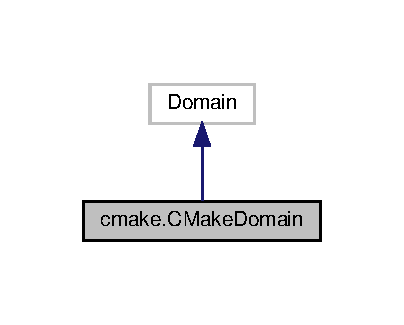
\includegraphics[width=194pt]{classcmake_1_1CMakeDomain__inherit__graph}
\end{center}
\end{figure}


Collaboration diagram for cmake.\+C\+Make\+Domain\+:
\nopagebreak
\begin{figure}[H]
\begin{center}
\leavevmode
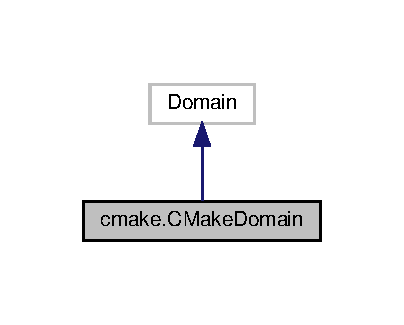
\includegraphics[width=194pt]{classcmake_1_1CMakeDomain__coll__graph}
\end{center}
\end{figure}
\subsection*{Public Member Functions}
\begin{DoxyCompactItemize}
\item 
def {\bfseries clear\+\_\+doc} (self, docname)\hypertarget{classcmake_1_1CMakeDomain_a2732fd39e980ef6d09b25eb900e5c4e4}{}\label{classcmake_1_1CMakeDomain_a2732fd39e980ef6d09b25eb900e5c4e4}

\item 
def {\bfseries resolve\+\_\+xref} (self, env, fromdocname, builder, typ, target, node, contnode)\hypertarget{classcmake_1_1CMakeDomain_a7c0d75227bf1e1745d43f6e19943b624}{}\label{classcmake_1_1CMakeDomain_a7c0d75227bf1e1745d43f6e19943b624}

\item 
def {\bfseries get\+\_\+objects} (self)\hypertarget{classcmake_1_1CMakeDomain_a0f5f539734ddf67f8ecf8dafe6003cd6}{}\label{classcmake_1_1CMakeDomain_a0f5f539734ddf67f8ecf8dafe6003cd6}

\end{DoxyCompactItemize}
\subsection*{Static Public Attributes}
\begin{DoxyCompactItemize}
\item 
string {\bfseries name} = \textquotesingle{}cmake\textquotesingle{}\hypertarget{classcmake_1_1CMakeDomain_a1f6d8b71882c94a479574702ce0428f1}{}\label{classcmake_1_1CMakeDomain_a1f6d8b71882c94a479574702ce0428f1}

\item 
string {\bfseries label} = \textquotesingle{}C\+Make\textquotesingle{}\hypertarget{classcmake_1_1CMakeDomain_a9215bbd38d25d788734f83dfc8c7f2bd}{}\label{classcmake_1_1CMakeDomain_a9215bbd38d25d788734f83dfc8c7f2bd}

\item 
dictionary {\bfseries object\+\_\+types}
\item 
dictionary {\bfseries directives}
\item 
dictionary {\bfseries roles}
\item 
dictionary {\bfseries initial\+\_\+data}
\end{DoxyCompactItemize}


\subsection{Detailed Description}
C\+Make domain. 



\subsection{Member Data Documentation}
\index{cmake\+::\+C\+Make\+Domain@{cmake\+::\+C\+Make\+Domain}!directives@{directives}}
\index{directives@{directives}!cmake\+::\+C\+Make\+Domain@{cmake\+::\+C\+Make\+Domain}}
\subsubsection[{\texorpdfstring{directives}{directives}}]{\setlength{\rightskip}{0pt plus 5cm}dictionary cmake.\+C\+Make\+Domain.\+directives\hspace{0.3cm}{\ttfamily [static]}}\hypertarget{classcmake_1_1CMakeDomain_a4ca0cbe98eb3a38b98df30377f550c08}{}\label{classcmake_1_1CMakeDomain_a4ca0cbe98eb3a38b98df30377f550c08}
{\bfseries Initial value\+:}
\begin{DoxyCode}
1 = \{
2         \textcolor{stringliteral}{'command'}:    CMakeObject,
3         \textcolor{stringliteral}{'variable'}:   CMakeObject,
4         \textcolor{comment}{# Other object types cannot be created except by the CMakeTransform}
5         \textcolor{comment}{# 'generator':  CMakeObject,}
6         \textcolor{comment}{# 'module':     CMakeObject,}
7         \textcolor{comment}{# 'policy':     CMakeObject,}
8         \textcolor{comment}{# 'prop\_cache': CMakeObject,}
9         \textcolor{comment}{# 'prop\_dir':   CMakeObject,}
10         \textcolor{comment}{# 'prop\_gbl':   CMakeObject,}
11         \textcolor{comment}{# 'prop\_inst':  CMakeObject,}
12         \textcolor{comment}{# 'prop\_sf':    CMakeObject,}
13         \textcolor{comment}{# 'prop\_test':  CMakeObject,}
14         \textcolor{comment}{# 'prop\_tgt':   CMakeObject,}
15         \textcolor{comment}{# 'manual':     CMakeObject,}
16     \}
\end{DoxyCode}
\index{cmake\+::\+C\+Make\+Domain@{cmake\+::\+C\+Make\+Domain}!initial\+\_\+data@{initial\+\_\+data}}
\index{initial\+\_\+data@{initial\+\_\+data}!cmake\+::\+C\+Make\+Domain@{cmake\+::\+C\+Make\+Domain}}
\subsubsection[{\texorpdfstring{initial\+\_\+data}{initial_data}}]{\setlength{\rightskip}{0pt plus 5cm}dictionary cmake.\+C\+Make\+Domain.\+initial\+\_\+data\hspace{0.3cm}{\ttfamily [static]}}\hypertarget{classcmake_1_1CMakeDomain_a471a8473fff4f5b8a3eae45e5ca0eea7}{}\label{classcmake_1_1CMakeDomain_a471a8473fff4f5b8a3eae45e5ca0eea7}
{\bfseries Initial value\+:}
\begin{DoxyCode}
1 = \{
2         \textcolor{stringliteral}{'objects'}: \{\},  \textcolor{comment}{# fullname -> docname, objtype}
3     \}
\end{DoxyCode}
\index{cmake\+::\+C\+Make\+Domain@{cmake\+::\+C\+Make\+Domain}!object\+\_\+types@{object\+\_\+types}}
\index{object\+\_\+types@{object\+\_\+types}!cmake\+::\+C\+Make\+Domain@{cmake\+::\+C\+Make\+Domain}}
\subsubsection[{\texorpdfstring{object\+\_\+types}{object_types}}]{\setlength{\rightskip}{0pt plus 5cm}dictionary cmake.\+C\+Make\+Domain.\+object\+\_\+types\hspace{0.3cm}{\ttfamily [static]}}\hypertarget{classcmake_1_1CMakeDomain_aed7e1d6464c1ee93cb9ec7deb5a44f52}{}\label{classcmake_1_1CMakeDomain_aed7e1d6464c1ee93cb9ec7deb5a44f52}
{\bfseries Initial value\+:}
\begin{DoxyCode}
1 = \{
2         \textcolor{stringliteral}{'command'}:    ObjType(\textcolor{stringliteral}{'command'},    \textcolor{stringliteral}{'command'}),
3         \textcolor{stringliteral}{'generator'}:  ObjType(\textcolor{stringliteral}{'generator'},  \textcolor{stringliteral}{'generator'}),
4         \textcolor{stringliteral}{'variable'}:   ObjType(\textcolor{stringliteral}{'variable'},   \textcolor{stringliteral}{'variable'}),
5         \textcolor{stringliteral}{'module'}:     ObjType(\textcolor{stringliteral}{'module'},     \textcolor{stringliteral}{'module'}),
6         \textcolor{stringliteral}{'policy'}:     ObjType(\textcolor{stringliteral}{'policy'},     \textcolor{stringliteral}{'policy'}),
7         \textcolor{stringliteral}{'prop\_cache'}: ObjType(\textcolor{stringliteral}{'prop\_cache'}, \textcolor{stringliteral}{'prop\_cache'}),
8         \textcolor{stringliteral}{'prop\_dir'}:   ObjType(\textcolor{stringliteral}{'prop\_dir'},   \textcolor{stringliteral}{'prop\_dir'}),
9         \textcolor{stringliteral}{'prop\_gbl'}:   ObjType(\textcolor{stringliteral}{'prop\_gbl'},   \textcolor{stringliteral}{'prop\_gbl'}),
10         \textcolor{stringliteral}{'prop\_inst'}:  ObjType(\textcolor{stringliteral}{'prop\_inst'},  \textcolor{stringliteral}{'prop\_inst'}),
11         \textcolor{stringliteral}{'prop\_sf'}:    ObjType(\textcolor{stringliteral}{'prop\_sf'},    \textcolor{stringliteral}{'prop\_sf'}),
12         \textcolor{stringliteral}{'prop\_test'}:  ObjType(\textcolor{stringliteral}{'prop\_test'},  \textcolor{stringliteral}{'prop\_test'}),
13         \textcolor{stringliteral}{'prop\_tgt'}:   ObjType(\textcolor{stringliteral}{'prop\_tgt'},   \textcolor{stringliteral}{'prop\_tgt'}),
14         \textcolor{stringliteral}{'manual'}:     ObjType(\textcolor{stringliteral}{'manual'},     \textcolor{stringliteral}{'manual'}),
15     \}
\end{DoxyCode}
\index{cmake\+::\+C\+Make\+Domain@{cmake\+::\+C\+Make\+Domain}!roles@{roles}}
\index{roles@{roles}!cmake\+::\+C\+Make\+Domain@{cmake\+::\+C\+Make\+Domain}}
\subsubsection[{\texorpdfstring{roles}{roles}}]{\setlength{\rightskip}{0pt plus 5cm}dictionary cmake.\+C\+Make\+Domain.\+roles\hspace{0.3cm}{\ttfamily [static]}}\hypertarget{classcmake_1_1CMakeDomain_a1a3a56c898d9720d688dea47de1715aa}{}\label{classcmake_1_1CMakeDomain_a1a3a56c898d9720d688dea47de1715aa}
{\bfseries Initial value\+:}
\begin{DoxyCode}
1 = \{
2         \textcolor{stringliteral}{'command'}:    CMakeXRefRole(fix\_parens = \textcolor{keyword}{True}, lowercase = \textcolor{keyword}{True}),
3         \textcolor{stringliteral}{'generator'}:  CMakeXRefRole(),
4         \textcolor{stringliteral}{'variable'}:   CMakeXRefRole(),
5         \textcolor{stringliteral}{'module'}:     CMakeXRefRole(),
6         \textcolor{stringliteral}{'policy'}:     CMakeXRefRole(),
7         \textcolor{stringliteral}{'prop\_cache'}: CMakeXRefRole(),
8         \textcolor{stringliteral}{'prop\_dir'}:   CMakeXRefRole(),
9         \textcolor{stringliteral}{'prop\_gbl'}:   CMakeXRefRole(),
10         \textcolor{stringliteral}{'prop\_inst'}:  CMakeXRefRole(),
11         \textcolor{stringliteral}{'prop\_sf'}:    CMakeXRefRole(),
12         \textcolor{stringliteral}{'prop\_test'}:  CMakeXRefRole(),
13         \textcolor{stringliteral}{'prop\_tgt'}:   CMakeXRefRole(),
14         \textcolor{stringliteral}{'manual'}:     CMakeXRefRole(),
15     \}
\end{DoxyCode}


The documentation for this class was generated from the following file\+:\begin{DoxyCompactItemize}
\item 
resources/sphinx/custom\+\_\+module/cmake.\+py\end{DoxyCompactItemize}

\hypertarget{classcmake_1_1CMakeModule}{}\section{cmake.\+C\+Make\+Module Class Reference}
\label{classcmake_1_1CMakeModule}\index{cmake.\+C\+Make\+Module@{cmake.\+C\+Make\+Module}}


Inheritance diagram for cmake.\+C\+Make\+Module\+:
\nopagebreak
\begin{figure}[H]
\begin{center}
\leavevmode
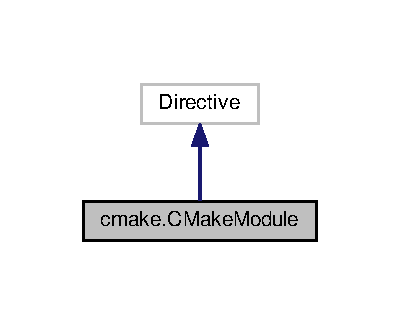
\includegraphics[width=192pt]{classcmake_1_1CMakeModule__inherit__graph}
\end{center}
\end{figure}


Collaboration diagram for cmake.\+C\+Make\+Module\+:
\nopagebreak
\begin{figure}[H]
\begin{center}
\leavevmode
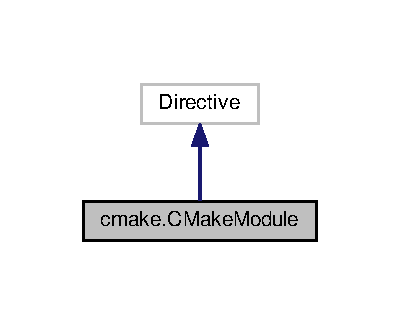
\includegraphics[width=192pt]{classcmake_1_1CMakeModule__coll__graph}
\end{center}
\end{figure}
\subsection*{Public Member Functions}
\begin{DoxyCompactItemize}
\item 
\mbox{\Hypertarget{classcmake_1_1CMakeModule_a42d2e41b69c92d05ff380fa12a5ff9c5}\label{classcmake_1_1CMakeModule_a42d2e41b69c92d05ff380fa12a5ff9c5}} 
def {\bfseries \+\_\+\+\_\+init\+\_\+\+\_\+} (self, args, keys)
\item 
\mbox{\Hypertarget{classcmake_1_1CMakeModule_a08741d315b312c41742816b16b8bfcef}\label{classcmake_1_1CMakeModule_a08741d315b312c41742816b16b8bfcef}} 
def {\bfseries run} (self)
\end{DoxyCompactItemize}
\subsection*{Public Attributes}
\begin{DoxyCompactItemize}
\item 
\mbox{\Hypertarget{classcmake_1_1CMakeModule_a8bdaac2e5425f8a443a797e31a2e3f24}\label{classcmake_1_1CMakeModule_a8bdaac2e5425f8a443a797e31a2e3f24}} 
{\bfseries re\+\_\+start}
\end{DoxyCompactItemize}
\subsection*{Static Public Attributes}
\begin{DoxyCompactItemize}
\item 
\mbox{\Hypertarget{classcmake_1_1CMakeModule_a8611294687a040b621ee65c24bdf4bf3}\label{classcmake_1_1CMakeModule_a8611294687a040b621ee65c24bdf4bf3}} 
int {\bfseries required\+\_\+arguments} = 1
\item 
\mbox{\Hypertarget{classcmake_1_1CMakeModule_a5b3ba9afdee1ce2a9ef4a4372804586b}\label{classcmake_1_1CMakeModule_a5b3ba9afdee1ce2a9ef4a4372804586b}} 
int {\bfseries optional\+\_\+arguments} = 0
\item 
\mbox{\Hypertarget{classcmake_1_1CMakeModule_a9101f08e555f3d9e7f45d766194bc50f}\label{classcmake_1_1CMakeModule_a9101f08e555f3d9e7f45d766194bc50f}} 
bool {\bfseries final\+\_\+argument\+\_\+whitespace} = True
\item 
\mbox{\Hypertarget{classcmake_1_1CMakeModule_adb45adc58cfd303e9efb70792cd2f7f4}\label{classcmake_1_1CMakeModule_adb45adc58cfd303e9efb70792cd2f7f4}} 
dictionary {\bfseries option\+\_\+spec} = \{\textquotesingle{}encoding\textquotesingle{}\+: directives.\+encoding\}
\end{DoxyCompactItemize}


The documentation for this class was generated from the following file\+:\begin{DoxyCompactItemize}
\item 
resources/sphinx/custom\+\_\+module/cmake.\+py\end{DoxyCompactItemize}

\hypertarget{classcmake_1_1CMakeObject}{}\section{cmake.\+C\+Make\+Object Class Reference}
\label{classcmake_1_1CMakeObject}\index{cmake.\+C\+Make\+Object@{cmake.\+C\+Make\+Object}}


Inheritance diagram for cmake.\+C\+Make\+Object\+:
\nopagebreak
\begin{figure}[H]
\begin{center}
\leavevmode
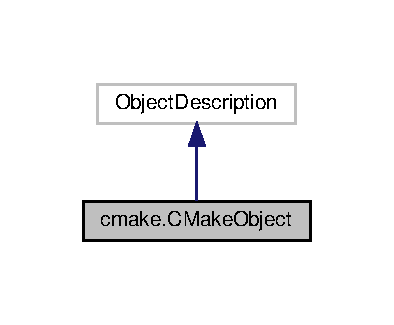
\includegraphics[width=189pt]{classcmake_1_1CMakeObject__inherit__graph}
\end{center}
\end{figure}


Collaboration diagram for cmake.\+C\+Make\+Object\+:
\nopagebreak
\begin{figure}[H]
\begin{center}
\leavevmode
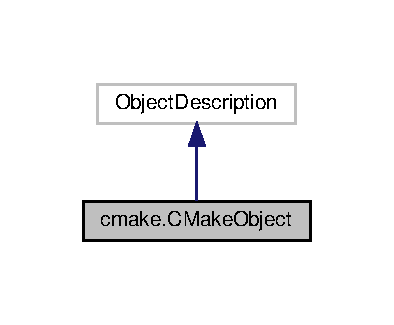
\includegraphics[width=189pt]{classcmake_1_1CMakeObject__coll__graph}
\end{center}
\end{figure}
\subsection*{Public Member Functions}
\begin{DoxyCompactItemize}
\item 
def {\bfseries handle\+\_\+signature} (self, sig, signode)\hypertarget{classcmake_1_1CMakeObject_a315ae4a1d65f1d45f0e77e146b31e80e}{}\label{classcmake_1_1CMakeObject_a315ae4a1d65f1d45f0e77e146b31e80e}

\item 
def {\bfseries add\+\_\+target\+\_\+and\+\_\+index} (self, name, sig, signode)\hypertarget{classcmake_1_1CMakeObject_a482e03d79771bd8937a47022b493f8bf}{}\label{classcmake_1_1CMakeObject_a482e03d79771bd8937a47022b493f8bf}

\end{DoxyCompactItemize}
\subsection*{Public Attributes}
\begin{DoxyCompactItemize}
\item 
{\bfseries objtype}\hypertarget{classcmake_1_1CMakeObject_a8e5fc4c75fdfb8b88fcbe6c37678cba5}{}\label{classcmake_1_1CMakeObject_a8e5fc4c75fdfb8b88fcbe6c37678cba5}

\end{DoxyCompactItemize}
\subsection*{Static Private Attributes}
\begin{DoxyCompactItemize}
\item 
{\bfseries \+\_\+re\+\_\+sub}\hypertarget{classcmake_1_1CMakeObject_a4a5c13fecd7ac9c0433b126f37a5806c}{}\label{classcmake_1_1CMakeObject_a4a5c13fecd7ac9c0433b126f37a5806c}

\end{DoxyCompactItemize}


The documentation for this class was generated from the following file\+:\begin{DoxyCompactItemize}
\item 
resources/sphinx/custom\+\_\+module/cmake.\+py\end{DoxyCompactItemize}

\hypertarget{classcmake_1_1CMakeTransform}{}\section{cmake.\+C\+Make\+Transform Class Reference}
\label{classcmake_1_1CMakeTransform}\index{cmake.\+C\+Make\+Transform@{cmake.\+C\+Make\+Transform}}


Inheritance diagram for cmake.\+C\+Make\+Transform\+:
\nopagebreak
\begin{figure}[H]
\begin{center}
\leavevmode
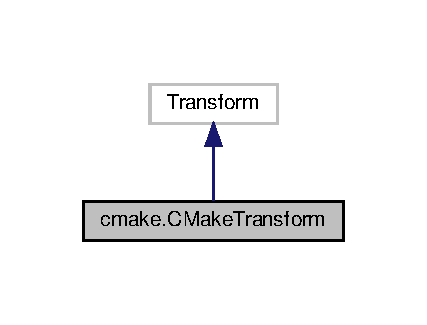
\includegraphics[width=205pt]{classcmake_1_1CMakeTransform__inherit__graph}
\end{center}
\end{figure}


Collaboration diagram for cmake.\+C\+Make\+Transform\+:
\nopagebreak
\begin{figure}[H]
\begin{center}
\leavevmode
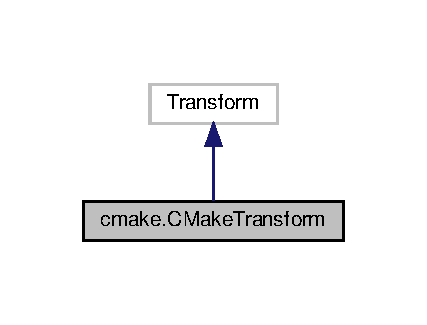
\includegraphics[width=205pt]{classcmake_1_1CMakeTransform__coll__graph}
\end{center}
\end{figure}
\subsection*{Public Member Functions}
\begin{DoxyCompactItemize}
\item 
\mbox{\Hypertarget{classcmake_1_1CMakeTransform_ac0c3ca6417777d94072b73cc31fceb5a}\label{classcmake_1_1CMakeTransform_ac0c3ca6417777d94072b73cc31fceb5a}} 
def {\bfseries \+\_\+\+\_\+init\+\_\+\+\_\+} (self, document, startnode)
\item 
def \hyperlink{classcmake_1_1CMakeTransform_aef2cd6c122395c8dd8c8a9a43c89be80}{parse\+\_\+title} (self, docname)
\begin{DoxyCompactList}\small\item\em Parse a document title as the first line starting in \mbox{[}A-\/\+Za-\/z0-\/9$<$\mbox{]} or fall back to the document basename if no such line exists. \end{DoxyCompactList}\item 
\mbox{\Hypertarget{classcmake_1_1CMakeTransform_ae75d969103bcd104f698ffe8bd764f9a}\label{classcmake_1_1CMakeTransform_ae75d969103bcd104f698ffe8bd764f9a}} 
def {\bfseries apply} (self)
\end{DoxyCompactItemize}
\subsection*{Public Attributes}
\begin{DoxyCompactItemize}
\item 
\mbox{\Hypertarget{classcmake_1_1CMakeTransform_a56d0ad5b508226202714d62125477210}\label{classcmake_1_1CMakeTransform_a56d0ad5b508226202714d62125477210}} 
{\bfseries titles}
\end{DoxyCompactItemize}
\subsection*{Static Public Attributes}
\begin{DoxyCompactItemize}
\item 
\mbox{\Hypertarget{classcmake_1_1CMakeTransform_ab5ae6cbdeb04d51d6bacbc516a27df80}\label{classcmake_1_1CMakeTransform_ab5ae6cbdeb04d51d6bacbc516a27df80}} 
int {\bfseries default\+\_\+priority} = 210
\end{DoxyCompactItemize}


\subsection{Member Function Documentation}
\mbox{\Hypertarget{classcmake_1_1CMakeTransform_aef2cd6c122395c8dd8c8a9a43c89be80}\label{classcmake_1_1CMakeTransform_aef2cd6c122395c8dd8c8a9a43c89be80}} 
\index{cmake\+::\+C\+Make\+Transform@{cmake\+::\+C\+Make\+Transform}!parse\+\_\+title@{parse\+\_\+title}}
\index{parse\+\_\+title@{parse\+\_\+title}!cmake\+::\+C\+Make\+Transform@{cmake\+::\+C\+Make\+Transform}}
\subsubsection{\texorpdfstring{parse\+\_\+title()}{parse\_title()}}
{\footnotesize\ttfamily def cmake.\+C\+Make\+Transform.\+parse\+\_\+title (\begin{DoxyParamCaption}\item[{}]{self,  }\item[{}]{docname }\end{DoxyParamCaption})}



Parse a document title as the first line starting in \mbox{[}A-\/\+Za-\/z0-\/9$<$\mbox{]} or fall back to the document basename if no such line exists. 

The cmake --help-\/$\ast$-\/list commands also depend on this convention. Return the title or False if the document file does not exist. 

The documentation for this class was generated from the following file\+:\begin{DoxyCompactItemize}
\item 
resources/sphinx/custom\+\_\+module/cmake.\+py\end{DoxyCompactItemize}

\hypertarget{classcmake_1_1CMakeXRefRole}{}\section{cmake.\+C\+Make\+X\+Ref\+Role Class Reference}
\label{classcmake_1_1CMakeXRefRole}\index{cmake.\+C\+Make\+X\+Ref\+Role@{cmake.\+C\+Make\+X\+Ref\+Role}}


Inheritance diagram for cmake.\+C\+Make\+X\+Ref\+Role\+:
\nopagebreak
\begin{figure}[H]
\begin{center}
\leavevmode
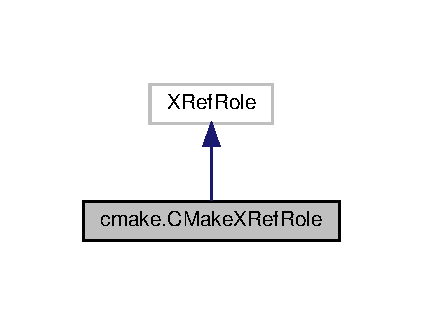
\includegraphics[width=203pt]{classcmake_1_1CMakeXRefRole__inherit__graph}
\end{center}
\end{figure}


Collaboration diagram for cmake.\+C\+Make\+X\+Ref\+Role\+:
\nopagebreak
\begin{figure}[H]
\begin{center}
\leavevmode
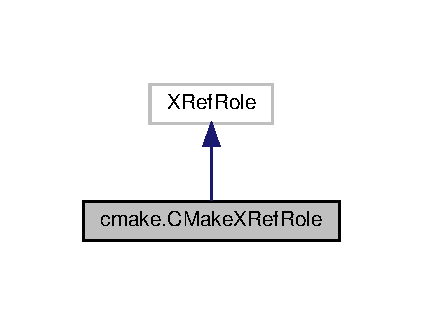
\includegraphics[width=203pt]{classcmake_1_1CMakeXRefRole__coll__graph}
\end{center}
\end{figure}
\subsection*{Public Member Functions}
\begin{DoxyCompactItemize}
\item 
def {\bfseries \+\_\+\+\_\+call\+\_\+\+\_\+} (self, typ, rawtext, text, args, keys)\hypertarget{classcmake_1_1CMakeXRefRole_ac1902f080ef5f30ca8ab71515d6e0024}{}\label{classcmake_1_1CMakeXRefRole_ac1902f080ef5f30ca8ab71515d6e0024}

\end{DoxyCompactItemize}
\subsection*{Static Private Attributes}
\begin{DoxyCompactItemize}
\item 
{\bfseries \+\_\+re}\hypertarget{classcmake_1_1CMakeXRefRole_aac6d8cdf12356ff1d7d8e71f3fc7b6d8}{}\label{classcmake_1_1CMakeXRefRole_aac6d8cdf12356ff1d7d8e71f3fc7b6d8}

\item 
{\bfseries \+\_\+re\+\_\+sub}\hypertarget{classcmake_1_1CMakeXRefRole_abee30c04841f76620a3f43cb01fd55a6}{}\label{classcmake_1_1CMakeXRefRole_abee30c04841f76620a3f43cb01fd55a6}

\end{DoxyCompactItemize}


The documentation for this class was generated from the following file\+:\begin{DoxyCompactItemize}
\item 
resources/sphinx/custom\+\_\+module/cmake.\+py\end{DoxyCompactItemize}

\hypertarget{classcmake_1_1CMakeXRefTransform}{}\section{cmake.\+C\+Make\+X\+Ref\+Transform Class Reference}
\label{classcmake_1_1CMakeXRefTransform}\index{cmake.\+C\+Make\+X\+Ref\+Transform@{cmake.\+C\+Make\+X\+Ref\+Transform}}


Inheritance diagram for cmake.\+C\+Make\+X\+Ref\+Transform\+:
\nopagebreak
\begin{figure}[H]
\begin{center}
\leavevmode
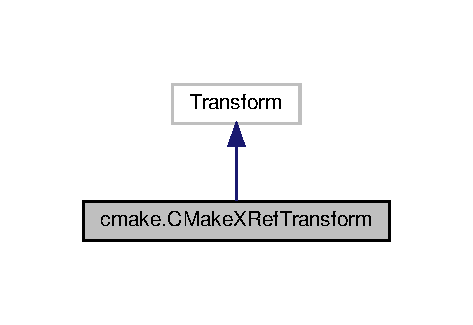
\includegraphics[width=227pt]{classcmake_1_1CMakeXRefTransform__inherit__graph}
\end{center}
\end{figure}


Collaboration diagram for cmake.\+C\+Make\+X\+Ref\+Transform\+:
\nopagebreak
\begin{figure}[H]
\begin{center}
\leavevmode
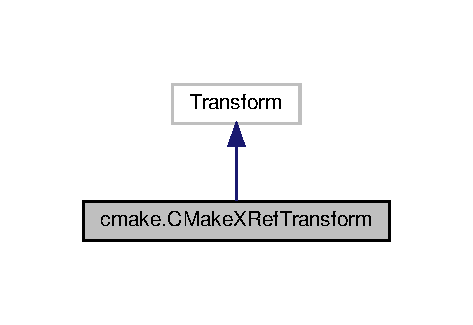
\includegraphics[width=227pt]{classcmake_1_1CMakeXRefTransform__coll__graph}
\end{center}
\end{figure}
\subsection*{Public Member Functions}
\begin{DoxyCompactItemize}
\item 
def {\bfseries apply} (self)\hypertarget{classcmake_1_1CMakeXRefTransform_a8727f9aa2814e7491695df2544981eb6}{}\label{classcmake_1_1CMakeXRefTransform_a8727f9aa2814e7491695df2544981eb6}

\end{DoxyCompactItemize}
\subsection*{Static Public Attributes}
\begin{DoxyCompactItemize}
\item 
int {\bfseries default\+\_\+priority} = 221\hypertarget{classcmake_1_1CMakeXRefTransform_ab2b872ed2d2e4d99bb3b50ae528c7955}{}\label{classcmake_1_1CMakeXRefTransform_ab2b872ed2d2e4d99bb3b50ae528c7955}

\end{DoxyCompactItemize}


The documentation for this class was generated from the following file\+:\begin{DoxyCompactItemize}
\item 
resources/sphinx/custom\+\_\+module/cmake.\+py\end{DoxyCompactItemize}

\hypertarget{classconf_1_1IfMode}{}\section{conf.\+If\+Mode Class Reference}
\label{classconf_1_1IfMode}\index{conf.\+If\+Mode@{conf.\+If\+Mode}}


Inheritance diagram for conf.\+If\+Mode\+:
\nopagebreak
\begin{figure}[H]
\begin{center}
\leavevmode
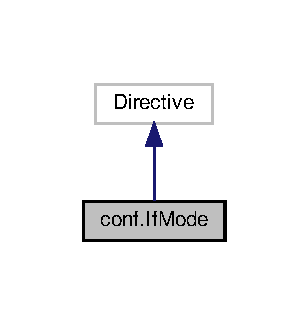
\includegraphics[width=148pt]{classconf_1_1IfMode__inherit__graph}
\end{center}
\end{figure}


Collaboration diagram for conf.\+If\+Mode\+:
\nopagebreak
\begin{figure}[H]
\begin{center}
\leavevmode
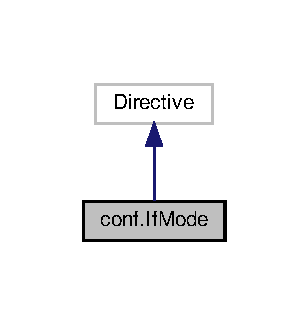
\includegraphics[width=148pt]{classconf_1_1IfMode__coll__graph}
\end{center}
\end{figure}
\subsection*{Public Member Functions}
\begin{DoxyCompactItemize}
\item 
\mbox{\Hypertarget{classconf_1_1IfMode_a8734a7a8ad5f3c9832d0856b8470871c}\label{classconf_1_1IfMode_a8734a7a8ad5f3c9832d0856b8470871c}} 
def {\bfseries run} (self)
\end{DoxyCompactItemize}
\subsection*{Static Public Attributes}
\begin{DoxyCompactItemize}
\item 
\mbox{\Hypertarget{classconf_1_1IfMode_aaea7225a5870ca4481d04f6ae781413f}\label{classconf_1_1IfMode_aaea7225a5870ca4481d04f6ae781413f}} 
bool {\bfseries has\+\_\+content} = True
\item 
\mbox{\Hypertarget{classconf_1_1IfMode_a6178050b552e80e923a467486ae3b6db}\label{classconf_1_1IfMode_a6178050b552e80e923a467486ae3b6db}} 
int {\bfseries required\+\_\+arguments} = 1
\item 
\mbox{\Hypertarget{classconf_1_1IfMode_a76d350d5aabb8c2dbdf47199a4b5b594}\label{classconf_1_1IfMode_a76d350d5aabb8c2dbdf47199a4b5b594}} 
int {\bfseries optional\+\_\+arguments} = 0
\item 
\mbox{\Hypertarget{classconf_1_1IfMode_aeb33a9725e6fc1216412d321cd46db09}\label{classconf_1_1IfMode_aeb33a9725e6fc1216412d321cd46db09}} 
bool {\bfseries final\+\_\+argument\+\_\+whitespace} = True
\item 
\mbox{\Hypertarget{classconf_1_1IfMode_a0e789bd8ead3911da5a47a2ed0f66cb7}\label{classconf_1_1IfMode_a0e789bd8ead3911da5a47a2ed0f66cb7}} 
dictionary {\bfseries option\+\_\+spec} = \{\}
\end{DoxyCompactItemize}


The documentation for this class was generated from the following file\+:\begin{DoxyCompactItemize}
\item 
resources/sphinx/sphinx/conf.\+py\end{DoxyCompactItemize}

\hypertarget{classconf_1_1SetMode}{}\section{conf.\+Set\+Mode Class Reference}
\label{classconf_1_1SetMode}\index{conf.\+Set\+Mode@{conf.\+Set\+Mode}}


Inheritance diagram for conf.\+Set\+Mode\+:
\nopagebreak
\begin{figure}[H]
\begin{center}
\leavevmode
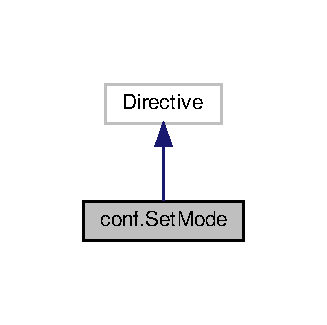
\includegraphics[width=157pt]{classconf_1_1SetMode__inherit__graph}
\end{center}
\end{figure}


Collaboration diagram for conf.\+Set\+Mode\+:
\nopagebreak
\begin{figure}[H]
\begin{center}
\leavevmode
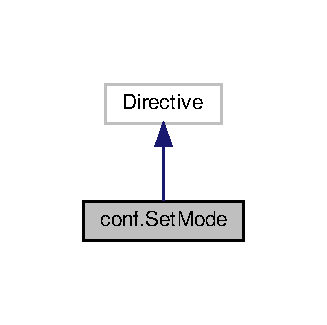
\includegraphics[width=157pt]{classconf_1_1SetMode__coll__graph}
\end{center}
\end{figure}
\subsection*{Public Member Functions}
\begin{DoxyCompactItemize}
\item 
\mbox{\Hypertarget{classconf_1_1SetMode_ac3e12cb0da9b23a8e299fbd202fa9253}\label{classconf_1_1SetMode_ac3e12cb0da9b23a8e299fbd202fa9253}} 
def {\bfseries run} (self)
\end{DoxyCompactItemize}
\subsection*{Static Public Attributes}
\begin{DoxyCompactItemize}
\item 
\mbox{\Hypertarget{classconf_1_1SetMode_ae1125c2c8ac3569a9e7189eaf36224ba}\label{classconf_1_1SetMode_ae1125c2c8ac3569a9e7189eaf36224ba}} 
bool {\bfseries has\+\_\+content} = False
\item 
\mbox{\Hypertarget{classconf_1_1SetMode_a33f8f61daab34475f5af93e15a3e3b5d}\label{classconf_1_1SetMode_a33f8f61daab34475f5af93e15a3e3b5d}} 
int {\bfseries required\+\_\+arguments} = 1
\item 
\mbox{\Hypertarget{classconf_1_1SetMode_abea8b1a21182e57d44ec6d36a1beac10}\label{classconf_1_1SetMode_abea8b1a21182e57d44ec6d36a1beac10}} 
int {\bfseries optional\+\_\+arguments} = 0
\item 
\mbox{\Hypertarget{classconf_1_1SetMode_a36cbd9320be885e5e096a5a4a3b065fd}\label{classconf_1_1SetMode_a36cbd9320be885e5e096a5a4a3b065fd}} 
bool {\bfseries final\+\_\+argument\+\_\+whitespace} = False
\end{DoxyCompactItemize}


The documentation for this class was generated from the following file\+:\begin{DoxyCompactItemize}
\item 
resources/sphinx/sphinx/conf.\+py\end{DoxyCompactItemize}

\chapter{File Documentation}
\hypertarget{____init_____8py}{}\section{python/mpi\+\_\+cmake\+\_\+modules/\+\_\+\+\_\+init\+\_\+\+\_\+.py File Reference}
\label{____init_____8py}\index{python/mpi\+\_\+cmake\+\_\+modules/\+\_\+\+\_\+init\+\_\+\+\_\+.\+py@{python/mpi\+\_\+cmake\+\_\+modules/\+\_\+\+\_\+init\+\_\+\+\_\+.\+py}}


\subsection{Detailed Description}
\begin{DoxyRefDesc}{License}
\item[\hyperlink{license__license000001}{License}]License B\+S\+D-\/3-\/\+Clause \end{DoxyRefDesc}
\begin{DoxyCopyright}{Copyright}
Copyright (c) 2019, New York University and Max Planck Gesellschaft. 
\end{DoxyCopyright}

\hypertarget{clang__format_8py}{}\section{python/mpi\+\_\+cmake\+\_\+modules/clang\+\_\+format.py File Reference}
\label{clang__format_8py}\index{python/mpi\+\_\+cmake\+\_\+modules/clang\+\_\+format.\+py@{python/mpi\+\_\+cmake\+\_\+modules/clang\+\_\+format.\+py}}
\subsection*{Namespaces}
\begin{DoxyCompactItemize}
\item 
 \hyperlink{namespacempi__cmake__modules_1_1clang__format_1_1py}{mpi\+\_\+cmake\+\_\+modules.\+clang\+\_\+format.\+py}
\begin{DoxyCompactList}\small\item\em Utility functions for creating formatting script based on clang. \end{DoxyCompactList}\end{DoxyCompactItemize}
\subsection*{Functions}
\begin{DoxyCompactItemize}
\item 
def \hyperlink{clang__format_8py_afe8dc8c8d15623fc93c48e51f5814787}{mpi\+\_\+cmake\+\_\+modules.\+clang\+\_\+format.\+find\+\_\+clang\+\_\+format} (name\+\_\+list=\mbox{[}\textquotesingle{}clang-\/format\textquotesingle{}\mbox{]})
\begin{DoxyCompactList}\small\item\em Find the full path to the clang-\/format executable. \end{DoxyCompactList}\item 
def \hyperlink{clang__format_8py_a9d5af1fa13452a51570bb28d245d5d79}{mpi\+\_\+cmake\+\_\+modules.\+clang\+\_\+format.\+load\+\_\+clang\+\_\+format\+\_\+config} ()
\begin{DoxyCompactList}\small\item\em Look for the clang-\/formt parameter file in this package. \end{DoxyCompactList}\item 
def \hyperlink{clang__format_8py_a9768c9300934448be2a773e8c8d2df0b}{mpi\+\_\+cmake\+\_\+modules.\+clang\+\_\+format.\+test\+\_\+valid\+\_\+file} (filename, extensions)
\begin{DoxyCompactList}\small\item\em Test if the input file exists and is of one of the provided extension. \end{DoxyCompactList}\item 
def \hyperlink{clang__format_8py_ad59764370ac726bc399da6336b6b64d3}{mpi\+\_\+cmake\+\_\+modules.\+clang\+\_\+format.\+get\+\_\+absolute\+\_\+path} (file\+\_\+or\+\_\+directory)
\begin{DoxyCompactList}\small\item\em Get the absolute path of a given path and check its existance. \end{DoxyCompactList}\item 
def \hyperlink{clang__format_8py_a45f75cf60b9373143390257a3ef49214}{mpi\+\_\+cmake\+\_\+modules.\+clang\+\_\+format.\+list\+\_\+of\+\_\+files\+\_\+to\+\_\+format} (files\+\_\+or\+\_\+directories, extensions)
\begin{DoxyCompactList}\small\item\em Get the list of files to format exploring the input arguments. \end{DoxyCompactList}\item 
def \hyperlink{clang__format_8py_aa7bc2c584f93ba6d7345a544824a146d}{mpi\+\_\+cmake\+\_\+modules.\+clang\+\_\+format.\+execute\+\_\+clang\+\_\+format} (clang\+\_\+format\+\_\+bin, clang\+\_\+format\+\_\+config, clang\+\_\+format\+\_\+arg)
\begin{DoxyCompactList}\small\item\em Execute the formatting of C/\+C++ files using clang-\/format. \end{DoxyCompactList}\end{DoxyCompactItemize}
\subsection*{Variables}
\begin{DoxyCompactItemize}
\item 
\mbox{\Hypertarget{clang__format_8py_a69c93a1da52a27430c5c942c41070465}\label{clang__format_8py_a69c93a1da52a27430c5c942c41070465}} 
{\bfseries mpi\+\_\+cmake\+\_\+modules.\+clang\+\_\+format.\+which} = distutils.\+spawn.\+find\+\_\+executable
\end{DoxyCompactItemize}


\subsection{Detailed Description}
\begin{DoxyRefDesc}{License}
\item[\hyperlink{license__license000002}{License}]License B\+S\+D-\/3-\/\+Clause \end{DoxyRefDesc}
\begin{DoxyCopyright}{Copyright}
Copyright (c) 2019, New York University and Max Planck Gesellschaft. 
\end{DoxyCopyright}


\subsection{Function Documentation}
\mbox{\Hypertarget{clang__format_8py_file_aa7bc2c584f93ba6d7345a544824a146d}\label{clang__format_8py_file_aa7bc2c584f93ba6d7345a544824a146d}} 
\index{clang\+\_\+format.\+py@{clang\+\_\+format.\+py}!execute\+\_\+clang\+\_\+format@{execute\+\_\+clang\+\_\+format}}
\index{execute\+\_\+clang\+\_\+format@{execute\+\_\+clang\+\_\+format}!clang\+\_\+format.\+py@{clang\+\_\+format.\+py}}
\subsubsection{\texorpdfstring{execute\+\_\+clang\+\_\+format()}{execute\_clang\_format()}}
{\footnotesize\ttfamily def mpi\+\_\+cmake\+\_\+modules.\+clang\+\_\+format.\+execute\+\_\+clang\+\_\+format (\begin{DoxyParamCaption}\item[{}]{clang\+\_\+format\+\_\+bin,  }\item[{}]{clang\+\_\+format\+\_\+config,  }\item[{}]{clang\+\_\+format\+\_\+arg }\end{DoxyParamCaption})}



Execute the formatting of C/\+C++ files using clang-\/format. 

Get the path to the executable, and run it using the clang-\/format insput parameter on the list of files to format.


\begin{DoxyParams}{Parameters}
{\em clang\+\_\+format\+\_\+bin} & Path to the clang-\/format binary.\\
\hline
{\em clang\+\_\+format\+\_\+config} & One line dictionnary string containing the clang-\/format parameters.\\
\hline
{\em clang\+\_\+format\+\_\+arg} & List of source files to parse. \\
\hline
\end{DoxyParams}
\mbox{\Hypertarget{clang__format_8py_file_afe8dc8c8d15623fc93c48e51f5814787}\label{clang__format_8py_file_afe8dc8c8d15623fc93c48e51f5814787}} 
\index{clang\+\_\+format.\+py@{clang\+\_\+format.\+py}!find\+\_\+clang\+\_\+format@{find\+\_\+clang\+\_\+format}}
\index{find\+\_\+clang\+\_\+format@{find\+\_\+clang\+\_\+format}!clang\+\_\+format.\+py@{clang\+\_\+format.\+py}}
\subsubsection{\texorpdfstring{find\+\_\+clang\+\_\+format()}{find\_clang\_format()}}
{\footnotesize\ttfamily def mpi\+\_\+cmake\+\_\+modules.\+clang\+\_\+format.\+find\+\_\+clang\+\_\+format (\begin{DoxyParamCaption}\item[{}]{name\+\_\+list = {\ttfamily \mbox{[}\textquotesingle{}clang-\/format\textquotesingle{}\mbox{]}} }\end{DoxyParamCaption})}



Find the full path to the clang-\/format executable. 

Look by default for the {\ttfamily clang-\/format} executable in the P\+A\+TH environment variable.


\begin{DoxyParams}{Parameters}
{\em name\+\_\+list} & list(str) {\ttfamily -\/-\/} Potential executable names which might differ according to the clang-\/format version available.\\
\hline
\end{DoxyParams}
\begin{DoxyReturn}{Returns}
The full path to the clang-\/format executable. 
\end{DoxyReturn}
\mbox{\Hypertarget{clang__format_8py_file_ad59764370ac726bc399da6336b6b64d3}\label{clang__format_8py_file_ad59764370ac726bc399da6336b6b64d3}} 
\index{clang\+\_\+format.\+py@{clang\+\_\+format.\+py}!get\+\_\+absolute\+\_\+path@{get\+\_\+absolute\+\_\+path}}
\index{get\+\_\+absolute\+\_\+path@{get\+\_\+absolute\+\_\+path}!clang\+\_\+format.\+py@{clang\+\_\+format.\+py}}
\subsubsection{\texorpdfstring{get\+\_\+absolute\+\_\+path()}{get\_absolute\_path()}}
{\footnotesize\ttfamily def mpi\+\_\+cmake\+\_\+modules.\+clang\+\_\+format.\+get\+\_\+absolute\+\_\+path (\begin{DoxyParamCaption}\item[{}]{file\+\_\+or\+\_\+directory }\end{DoxyParamCaption})}



Get the absolute path of a given path and check its existance. 

Check if file\+\_\+or\+\_\+directory is an existing file or directory, if so, returns it. Otherwise, assumes it is a relative path, which it upgrades to an absolute path, this it returns. If the upgraded path does not correspond to an existing file or directory, returns None


\begin{DoxyParams}{Parameters}
{\em file\+\_\+or\+\_\+directory} & str {\ttfamily -\/-\/} a relative or an absolute path\\
\hline
\end{DoxyParams}
\begin{DoxyReturn}{Returns}
an absolute existing path (str) or None 
\end{DoxyReturn}
\mbox{\Hypertarget{clang__format_8py_file_a45f75cf60b9373143390257a3ef49214}\label{clang__format_8py_file_a45f75cf60b9373143390257a3ef49214}} 
\index{clang\+\_\+format.\+py@{clang\+\_\+format.\+py}!list\+\_\+of\+\_\+files\+\_\+to\+\_\+format@{list\+\_\+of\+\_\+files\+\_\+to\+\_\+format}}
\index{list\+\_\+of\+\_\+files\+\_\+to\+\_\+format@{list\+\_\+of\+\_\+files\+\_\+to\+\_\+format}!clang\+\_\+format.\+py@{clang\+\_\+format.\+py}}
\subsubsection{\texorpdfstring{list\+\_\+of\+\_\+files\+\_\+to\+\_\+format()}{list\_of\_files\_to\_format()}}
{\footnotesize\ttfamily def mpi\+\_\+cmake\+\_\+modules.\+clang\+\_\+format.\+list\+\_\+of\+\_\+files\+\_\+to\+\_\+format (\begin{DoxyParamCaption}\item[{}]{files\+\_\+or\+\_\+directories,  }\item[{}]{extensions }\end{DoxyParamCaption})}



Get the list of files to format exploring the input arguments. 

Explore recursively the directories given in the input list and create a list of all files. Add to this list the files given in the input list. Sort out the files that are source-\/files or not and return the list of source files.


\begin{DoxyParams}{Parameters}
{\em files\+\_\+or\+\_\+directories} & list(str) {\ttfamily -\/-\/} List of files or directories.\\
\hline
{\em extensions} & list(str) {\ttfamily -\/-\/} List of extensions to check against\\
\hline
\end{DoxyParams}
\begin{DoxyReturn}{Returns}
True if the file ends with one of the given extensions, typically\+: 
\begin{DoxyCode}
(\textcolor{stringliteral}{".h"}, \textcolor{stringliteral}{".c"}, \textcolor{stringliteral}{".hh"}, \textcolor{stringliteral}{".cc"}, \textcolor{stringliteral}{".hpp"}, \textcolor{stringliteral}{".cpp"}, \textcolor{stringliteral}{".hxx"}, \textcolor{stringliteral}{".cxx"})
\end{DoxyCode}
 False otherwise. 
\end{DoxyReturn}
\mbox{\Hypertarget{clang__format_8py_file_a9d5af1fa13452a51570bb28d245d5d79}\label{clang__format_8py_file_a9d5af1fa13452a51570bb28d245d5d79}} 
\index{clang\+\_\+format.\+py@{clang\+\_\+format.\+py}!load\+\_\+clang\+\_\+format\+\_\+config@{load\+\_\+clang\+\_\+format\+\_\+config}}
\index{load\+\_\+clang\+\_\+format\+\_\+config@{load\+\_\+clang\+\_\+format\+\_\+config}!clang\+\_\+format.\+py@{clang\+\_\+format.\+py}}
\subsubsection{\texorpdfstring{load\+\_\+clang\+\_\+format\+\_\+config()}{load\_clang\_format\_config()}}
{\footnotesize\ttfamily def mpi\+\_\+cmake\+\_\+modules.\+clang\+\_\+format.\+load\+\_\+clang\+\_\+format\+\_\+config (\begin{DoxyParamCaption}{ }\end{DoxyParamCaption})}



Look for the clang-\/formt parameter file in this package. 

Look for the \+\_\+clang-\/format file located in this package and convert it in a one line dictionnary string.

\begin{DoxyReturn}{Returns}
The \+\_\+clang-\/format in a online dictionnary string. 
\end{DoxyReturn}
\mbox{\Hypertarget{clang__format_8py_file_a9768c9300934448be2a773e8c8d2df0b}\label{clang__format_8py_file_a9768c9300934448be2a773e8c8d2df0b}} 
\index{clang\+\_\+format.\+py@{clang\+\_\+format.\+py}!test\+\_\+valid\+\_\+file@{test\+\_\+valid\+\_\+file}}
\index{test\+\_\+valid\+\_\+file@{test\+\_\+valid\+\_\+file}!clang\+\_\+format.\+py@{clang\+\_\+format.\+py}}
\subsubsection{\texorpdfstring{test\+\_\+valid\+\_\+file()}{test\_valid\_file()}}
{\footnotesize\ttfamily def mpi\+\_\+cmake\+\_\+modules.\+clang\+\_\+format.\+test\+\_\+valid\+\_\+file (\begin{DoxyParamCaption}\item[{}]{filename,  }\item[{}]{extensions }\end{DoxyParamCaption})}



Test if the input file exists and is of one of the provided extension. 


\begin{DoxyParams}{Parameters}
{\em filename} & Path to the file to test.\\
\hline
{\em extensions} & iterable of accepted extensions.\\
\hline
\end{DoxyParams}
\begin{DoxyReturn}{Returns}
True if the file exits and ends with one of the extension.
\end{DoxyReturn}
False otherwise. 
\hypertarget{yaml2oneline_8py}{}\section{python/mpi\+\_\+cmake\+\_\+modules/yaml2oneline.py File Reference}
\label{yaml2oneline_8py}\index{python/mpi\+\_\+cmake\+\_\+modules/yaml2oneline.\+py@{python/mpi\+\_\+cmake\+\_\+modules/yaml2oneline.\+py}}
\subsection*{Namespaces}
\begin{DoxyCompactItemize}
\item 
 \hyperlink{namespacempi__cmake__modules_1_1yaml2oneline}{mpi\+\_\+cmake\+\_\+modules.\+yaml2oneline}
\begin{DoxyCompactList}\small\item\em Convert a Y\+A\+ML file in a one line string. \end{DoxyCompactList}\end{DoxyCompactItemize}
\subsection*{Functions}
\begin{DoxyCompactItemize}
\item 
def \hyperlink{namespacempi__cmake__modules_1_1yaml2oneline_a82021b35eab75040f7372ecfd4f21b0d}{mpi\+\_\+cmake\+\_\+modules.\+yaml2oneline.\+yaml2oneline} (filename)
\begin{DoxyCompactList}\small\item\em Convert a yaml file into a dictionnary one-\/line string. \end{DoxyCompactList}\end{DoxyCompactItemize}
\subsection*{Variables}
\begin{DoxyCompactItemize}
\item 
\mbox{\Hypertarget{namespacempi__cmake__modules_1_1yaml2oneline_ac27969d1fd9b275701d6a253c87c6eb1}\label{namespacempi__cmake__modules_1_1yaml2oneline_ac27969d1fd9b275701d6a253c87c6eb1}} 
\hyperlink{namespacempi__cmake__modules_1_1yaml2oneline_ac27969d1fd9b275701d6a253c87c6eb1}{mpi\+\_\+cmake\+\_\+modules.\+yaml2oneline.\+filename} = sys.\+argv\mbox{[}1\mbox{]}
\begin{DoxyCompactList}\small\item\em input yaml file name \end{DoxyCompactList}\end{DoxyCompactItemize}


\subsection{Detailed Description}
\begin{DoxyRefDesc}{License}
\item[\hyperlink{license__license000003}{License}]License B\+S\+D-\/3-\/\+Clause \end{DoxyRefDesc}
\begin{DoxyCopyright}{Copyright}
Copyright (c) 2019, New York University and Max Planck Gesellschaft. 
\end{DoxyCopyright}

\hypertarget{setup_8py}{}\section{setup.\+py File Reference}
\label{setup_8py}\index{setup.\+py@{setup.\+py}}


This file defines the python modules in this package.  


\subsection*{Namespaces}
\begin{DoxyCompactItemize}
\item 
 \hyperlink{namespacedynamic__graph__manager}{dynamic\+\_\+graph\+\_\+manager}
\begin{DoxyCompactList}\small\item\em Example of hardware communication client based on R\+OS. \end{DoxyCompactList}\end{DoxyCompactItemize}
\subsection*{Variables}
\begin{DoxyCompactItemize}
\item 
{\bfseries setup.\+setup\+\_\+args} = generate\+\_\+distutils\+\_\+setup()\hypertarget{setup_8py_a504ffa482edfe0eff08f64b2f5dff0e9}{}\label{setup_8py_a504ffa482edfe0eff08f64b2f5dff0e9}

\end{DoxyCompactItemize}


\subsection{Detailed Description}
This file defines the python modules in this package. 

\begin{DoxyAuthor}{Author}
Maximilien Naveau (\href{mailto:maximilien.naveau@gmail.com}{\tt maximilien.\+naveau@gmail.\+com}) 
\end{DoxyAuthor}
\begin{DoxyRefDesc}{License}
\item[\hyperlink{license__license000042}{License}]License B\+S\+D-\/3-\/\+Clause \end{DoxyRefDesc}
\begin{DoxyCopyright}{Copyright}
Copyright (c) 2019, New York University and Max Planck Gesellschaft. 
\end{DoxyCopyright}
\begin{DoxyDate}{Date}
2019-\/05-\/22 
\end{DoxyDate}

%--- End generated contents ---

% Index
\backmatter
\newpage
\phantomsection
\clearemptydoublepage
\addcontentsline{toc}{chapter}{Index}
\printindex

\end{document}
